%%%%%%%%%%%%%%%%%%%%%%%%%%%%%%%%%%%%%%%%%%%%%%%%%%%%%%%%%%%%%%%%%%%%%%%%%%%%
%% Trim Size: 9.75in x 6.5in
%% Text Area: 8in (include Runningheads) x 5in
%% ws-ijfe.tex   :   8-11-05
%% Tex file to use with ws-ijm.cls written in Latex2E.
%% The content, structure, format and layout of this style file is the
%% property of World Scientific Publishing Co. Pte. Ltd.
%% Copyright 1995, 2002 by World Scientific Publishing Co.
%% All rights are reserved.
%%%%%%%%%%%%%%%%%%%%%%%%%%%%%%%%%%%%%%%%%%%%%%%%%%%%%%%%%%%%%%%%%%%%%%%%%%%%
%

\documentclass{ws-ijfe}

%%% standard pachages
\usepackage{ amsmath, amssymb, amsfonts, graphicx, epsfig, mathtools, epstopdf}
%%%
\usepackage[section]{placeins}
\usepackage{morefloats}
\usepackage{float}
%%%%%%%%%%%%%%%%%%%%%%%%%%%%%%%%%%%%
%%% pachage to write Indicator function as 'blackboard bold 1': \mathbbm{1}. Made a custom macro \1=\mathbbm{1}
\usepackage{bbm}
%%%%%%%%%%%%%%%%%%%%%%%%%%%%%%%%%%%%

%%%%%%%%%%%%%%%%%%%%%%%%%%%%%%%%%%%%
% This package gives the enumerate environment an optional argument
% which determines the style in which the counter is printed.
% http://www.ctex.org/documents/packages/table/enumerate.pdf
\usepackage{enumerate}
%%%%%%%%%%%%%%%%%%%%%%%%%%%%%%%%%%%%

% to use strike out \sout
\usepackage[normalem]{ulem}


%%%%%%%%%%%%%%%%%%%%%%%%%%%%%%%%%%%%
% To display the labels used in a tex file in the dvi file (for example, if a theorem is labelled with the \label command) use the package
%\usepackage{showkeys}
%This will display all labels (for example, in the case of a labelled theorem, the label of the theorem will occur in the margin of the dvi file.
%The command above by itself not only displays labels when they are first named but also when they are cited (or referenced). To disable this feature use the following %options with the showkeys package
%\usepackage[notref, notcite]{showkeys}
%%%%%%%%%%%%%%%%%%%%%%%%%%%%%%%%%%%%


%%%%%%%%%%%%%%%%%%%%%%%%%%%%%%%%%%%%
% It extends the functionality of all the LATEX cross-referencing commands (including the table of contents, bibliographies etc) to produce \special commands which a driver can turn into hypertext links; it also provides new commands to allow the user to write ad hoc hypertext links, including those to external documents and URLs.
% http://www.tug.org/applications/hyperref/manual.html
\usepackage[colorlinks=true, pdfstartview=FitV, linkcolor=blue,
            citecolor=blue, urlcolor=blue]{hyperref}
\usepackage[usenames]{color}
\definecolor{Red}{rgb}{0.7,0,0.1}
\definecolor{Green}{rgb}{0,0.7,0}
%%%%%%%%%%%%%%%%%%%%%%%%%%%%%%%%%%%%


%%%%%%%%%%%%%%%%%%%%%%%%%%%%%%%%%%%%
% It is a LaTeX package to act as generalized
% interface for standard and non-standard bibliographic style files (BibTeX).
% http://www.ctan.org/tex-archive/macros/latex/contrib/natbib/
%\usepackage[numbers]{natbib}
%\usepackage{natbib}
%%%%%%%%%%%%%%%%%%%%%%%%%%%%%%%%%%%%


%%%%%%%%%%%%%%%%%%%%%%%%%%%%%%%%%%%%
% a good looking way to format urls
% http://mirror.its.uidaho.edu/pub/tex-archive/help/Catalogue/entries/url.html
\usepackage{url}
% Define a new 'leo' style for the package that will use a smaller font.
\makeatletter\def\url@leostyle{%
 \@ifundefined{selectfont}{\def\UrlFont{\sf}}{\def\UrlFont{\scriptsize\ttfamily}}} \makeatother\urlstyle{leo}
%%%%%%%%%%%%%%%%%%%%%%%%%%%%%%%%%%%%%

% to add accents and comments
%\usepackage{ comment}


%% custom margins
%\def\baselinestretch{1.1}
\setlength{\voffset}{-0.5in}
\setlength{\hoffset}{-0.5in}
\setlength{\textheight}{8.5in}
\setlength{\textwidth}{6in}
%% or use geometry pacakge
%\usepackage[margin=1.1in, dvips, letterpaper]{geometry}


%%%%%%%%%%%%%%%%%%%%%%%%%%%%%%%%%%%%%
%\newtheorem{theorem}{Theorem}[section]
%\newtheorem{proposition}[theorem]{Proposition}
%\newtheorem{lemma}{Lemma}[section]
%\newtheorem{corollary}[theorem]{Corollary}

%\theoremstyle{definition}
%\newtheorem{definition}[theorem]{Definition}
%\newtheorem{definition}{Definition}[section]
%\newtheorem{example}[theorem]{Example}
%\newtheorem{example}{Example}[section]
%\theoremstyle{remark}
%\newtheorem{remark}[theorem]{Remark}

%\newtheoremstyle{dotless}{}{}{\itshape}{}{\bfseries}{}{ }{}
%\theoremstyle{dotless}
%\newtheorem{assumption}{Assumption}
%\renewcommand*{\theassumption}{(\Alph{assumption})}
%\numberwithin{equation}{section}
%\numberwithin{theorem}{section}
%\renewcommand{\labelitemi}{ {\small $\rhd$}}

%%%%%%%%%%%%%%%%%%%%%%%%%%%%%%%%%%%%%
%%% used for editing and making comments in color
% Example \ig{Remarks and Commets}
\newcommand{\ti}[1]{\textcolor[rgb]{0.00, 0.0, 0.98}{T\&I: #1} }
\newcommand{\ig}[1]{\textcolor[rgb]{1.00, 0.0, 0.98}{Ig: #1} }
\newcommand{\ii}[1]{\textcolor[rgb]{0.00, 0.60, 0.5}{II: #1} }
\newcommand{\rr}[1]{\textcolor[rgb]{0.00, 0.65, 0}{RR: #1} }
\newcommand{\trb}[1]{\textcolor[rgb]{1.00, 0.00, 0}{TRB: #1} }
%%%%%%%%%%%%%%%%%%%%%%%%%%%%%%%%%%%%%


%%%%%%%%%%%%%%%%%%%%%%%%%%%%%%%%%%%%%
%%%     Igor's macros
%% \mathcal Letters
\def\cA{\mathcal{A}}
\def\cB{\mathcal{B}}
\def\cC{\mathcal{C}}
\def\cD{\mathcal{D}}
\def\cE{\mathcal{E}}
\def\cF{\mathcal{F}}
\def\cG{\mathcal{G}}
\def\cH{\mathcal{H}}
\def\cI{\mathcal{I}}
\def\cJ{\mathcal{J}}
\def\cK{\mathcal{K}}
\def\cL{\mathcal{L}}
\def\cM{\mathcal{M}}
\def\cN{\mathcal{N}}
\def\cO{\mathcal{O}}
\def\cP{\mathcal{P}}
\def\cQ{\mathcal{Q}}
\def\cR{\mathcal{R}}
\def\cS{\mathcal{S}}
\def\cT{\mathcal{T}}
\def\cU{\mathcal{U}}
\def\cV{\mathcal{V}}
\def\cW{\mathcal{W}}
\def\cX{\mathcal{X}}
\def\cY{\mathcal{Y}}
\def\cZ{\mathcal{Z}}

%% \mathbb Letters
\def\bA{\mathbb{A}}
\def\bB{\mathbb{B}}
\def\bC{\mathbb{C}}
\def\bD{\mathbb{D}}
\def\bE{\mathbb{E}}
\def\bF{\mathbb{F}}
\def\bG{\mathbb{G}}
\def\bH{\mathbb{H}}
\def\bI{\mathbb{I}}
\def\bJ{\mathbb{J}}
\def\bK{\mathbb{K}}
\def\bL{\mathbb{L}}
\def\bM{\mathbb{M}}
\def\bN{\mathbb{N}}
\def\bO{\mathbb{O}}
\def\bP{\mathbb{P}}
\def\bQ{\mathbb{Q}}
\def\bR{\mathbb{R}}
\def\bS{\mathbb{S}}
\def\bT{\mathbb{T}}
\def\bU{\mathbb{U}}
\def\bV{\mathbb{V}}
\def\bW{\mathbb{W}}
\def\bX{\mathbb{X}}
\def\bY{\mathbb{Y}}
\def\bZ{\mathbb{Z}}

\def\I{\mathbb{I}}
\def\1{\mathbbm{1}}


\newcommand{\pd}[1]{\partial_{#1}}      % partial derivative
\newcommand{\indFn}[1]{1 \! \! 1_{#1}}  % indicator function
\newcommand{\set}[1]{\left\{#1\right\}} % set: {xyz}
\renewcommand{\mid}{\;|\;}              % mid bar with small spaces before and after: x | y
\newcommand{\Mid}{\;\Big | \;}          % big bar with small spaces before and after:

\DeclareMathOperator*{\esssup}{ess\,sup} % ess sup
\DeclareMathOperator*{\essinf}{ess\,inf} % ess inf
\DeclareMathOperator*{\argmin}{arg\,min} % argmin
\DeclareMathOperator*{\argmax}{arg\,max} % argmax
%%%%%%%%%%%%%%%%%%%%%%%%%%%%%%%%%%%%%

%%%%%% d for derivative
\def\d{\mathrm{d}} 

\usepackage{graphicx}
\usepackage{cleveref}
\graphicspath{ {graphs/} }
\newcommand\numberthis{\addtocounter{equation}{1}\tag{\theequation}}
\renewcommand{\thefootnote}{\arabic{footnote}}
\usepackage{multirow}
\usepackage{threeparttable}



\begin{document}

\markboth{Authors' Names}
{Instructions for Typesetting Camera-Ready Manuscripts}

%%%%%%%%%%%%%%%%%%%%% Publisher's Area please ignore %%%%%%%%%%%%%%
\catchline{}{}{}{}{}
%%%%%%%%%%%%%%%%%%%%%%%%%%%%%%%%%%%%%%%%%%%%%%%%%%%%%%%%%%%%%%%%%%%

\title{Computing Option Prices Based on Heston Model to a Specified Tolerance\footnote{Typeset title in
10~pt Times Roman uppercase and boldface. Please write
down in pencil a short title to be used as the running head.}}

\author{Xiaoyang Zhao\footnote{xzhao31@hawk.iit.edu}, Tianci Zhu\footnote{tianci.zhu26@gmail.com} and Fred J. Hickernel\footnote{hickernell@iit.edu, 312.567.8983}l\footnote{Typeset names in 8~pt Times Roman, uppercase and lightface.  Use footnotes only to indicate if permanent and present addresses are different. Funding information should go in the Acknowledgement section.}}

\address{\footnote{Typeset
affiliation and mailing addresses in 8pt Times italic.} \\
10 W. 32rd Street, Chicago IL 60616\\Department of Applied Mathematics\\Illinois Institute of Technology}

%\author{OTHER D. AUTHOR}

%\address{Full affiliations \\
%,mailing addresses and telephone number}

\maketitle

\begin{abstract}
 The Quadratic Exponential (QE) model is a market standard simulation method for the Heston stochastic volatility model. We identify certain numerical problems with the standard discretization and modify the original method to correct these problems. We implement our modified QE scheme for the Heston model in the Guaranteed Automatic Integration Library (GAIL)---a suite of algorithms that includes Monte Carlo and quasi-Monte Carlo methods for multidimensional integration and computation of means. GAIL computes answers to satisfy user-defined error tolerances. We also implement variance reduction techniques for our modified QE scheme in GAIL. The numerical results show that our modified scheme is fast and accurate, and satisfies the user-defined error tolerances.

%Include a one-paragraph abstract of no more than 100 words. Do not include references, footnotes, or abbreviations in the abstract. Typeset the abstract in 8 pt Times Roman with baselineskip of 10 pt, making an indentation of $\frac14$ inch on the left and right margins. Typeset similarly for keywords below.
\end{abstract}

\keywords{ Enclose with each manuscript, on a separate page, from three to five keywords. }

\section{Introduction}

In the financial market, observed volatility of the asset prices is not a constant. For more accurate option pricing, we need an algorithm that simulates the volatility process. There are several well-known stochastic volatility models: the Hull-white model \cite{HullWhite1987}, the Scott-Chesny model \cite{ScottChesney1989}, the Heston model \cite{Heston1993} and the SABR model \cite{SABR2002}. We focus on the Heston model since it is one of the most widely used stochastic volatility models. Specifically, the Quadratic Exponential (QE) scheme is used to simulate the volatility process and the Broadie-Kaya scheme gives the discretization of the asset price process.

However, the standard implementation gives inaccurate results when the volatility of the asset prices' variance is very small or zero. Thus inaccuracy is accentuated when the initial variance does not start from the value of the long-term variance. We identify this problem and fix it by finding a more accurate approximation of the time integral of the volatility. We also make a change of variables in the QE scheme to avoid round-off errors in the discretization scheme of the asset price process. We compare the results with different options at different strike prices. Our numerical experiments show that the new algorithm is accurate and fast. %In addition, we implement the modified scheme in the Guaranteed Automatic Integration Library (GAIL), which theoretically guarantees the result and stops algorithms automatically with user defined error tolerance. %We compare the results with other simulation methods such as geometric Brownian motion and quasi-Monte Carlo, when setting the volatility of asset prices' volatility as zero, because in this case, the algorithm works like the one of asset price process with deterministic volatility. It shows that the new algorithm is accurate and fast.

In addition, we implement the modified scheme in the Guaranteed Automatic Integration Library (GAIL), which theoretically guarantees the result and stops algorithms automatically with user defined error tolerance. The GAIL includes a suite of algorithms that applies the Monte Carlo methods for multidimensional integration and computation of means. The financial application modules of GAIL are under construction, and our work is aimed to add efficient and accurate algorithms of calculating stochastic volatility model in the asset path class.

The QE model was developed by \cite{Andersen2006}. It is a market standard simulation method for the Heston model. Its attractiveness lies in its efficiency. It relies on simple probability density functions and needs a moderate amount of storage. Depending on the value of the volatility of the variance, the QE scheme approximates its distribution using either Gaussian or exponential distribution. After obtaining the value of the volatility at each time step, the Broadie-Kaya scheme is used to simulate the dynamics of the asset price process. The Broadie-Kaya scheme does not satisfy an equivalent discrete-time martingale condition. The martingale property can be attained by adjusting the Broadie-Kaya scheme.

The setup of the paper is as follows: we first introduce Heston model, QE scheme and the Broadie-Kaya scheme. Then, we derive our modified QE algorithm and provide its justification. After that, we explain variance reduction techniques and present numerical tests. At last, we summarize our work and discuss possible future work.

\section{Options Modeled by the Heston Stochastic Volatility Model}
\subsection{The Heston model}
Steven L. Heston introduced a stochastic volatility model which describes the evolution of the volatility of an asset price process \cite{Heston1993}. Compared to fixed volatility models, stochastic volatility models more accurately explain data from the real world.
The Heston model assumes the following dynamics of stock price and volatility processes:
 \begin{align}
    \d X_t & =\mu X_t\,\d t+\sqrt{V_t}X_t\,\d W_t^1\label{eq1}\\
    \d V_t &= \kappa (\theta-V_t)\,\d t +\nu\sqrt{V_t}\,\d W_t^2\label{eq2}
  \end{align}

The first equation describes the asset price process $X_t$ and the second equation gives the evolution of the variance process $V_t$. Two standard Brownian motions, $\d W_1$ and $\d W_2$, are set with a correlation constant $\rho$. The drift, the mean reversion speed of the variance, the long-term variance, and the volatility of the variance are denoted by $\mu$, $\kappa$, $\theta$ and $\nu$ respectively.

%\begin{align*}
%\text{where }&\\
%   & X\text{ is the asset price process}\\
%   & V\text{ is the stochastic volatility process}\\
%   & \d W_1 \text{ and } \d W_2 \text{ are two standard Brownian motions which are correlated}\\
%   &\rho \text{ is the correlation,} \\
%   & \mu \text{ is the the risk-free interest rate,}\\%r \text{ and } d \text{ are respectively the continuously compounded risk-free interest rate and dividend yield,}  \\
%   & \kappa \text{ is the speed of mean reversion,} \\
%   & \theta \text{ is the value of the long-term variance,} \\
%   & \nu \text{ is the volatility of volatility.}
%\end{align*}

Applying the Ito's formula to Eq.\eqref{eq1}, we have an equivalent form of asset price process:.
\begin{equation}\label{logX}
  \d\ln(X)=(\mu-\frac{V}{2})\,\d t+\sqrt{V}\,\d W_1
\end{equation}

The asset price process $X$ is governed by a geometric Brownian motion stochastic volatility.

\subsection{The quadratic exponential scheme for stochastic volatility}\label{se:QE}
We apply the Quadratic Exponential Scheme illustrated in Andersen (2006) \cite{Andersen} to simulate the volatility process. Let $\hat{V}$ denote the discrete-time approximation of $V$. Detailed steps are listed below.

\begin{enumerate}
\item Given $\hat{V_t}$, compute $m$ and $s^2$ from following equations
\begin{align*}
  m &=\theta + (\hat{V_t}-\theta)e^{-\kappa\Delta} \\
  s^2 &=\frac{\hat{V_t}\nu^2 e^{-\kappa\Delta}}{\kappa}\bigg(1-e^{-\kappa\Delta}\bigg)+\frac{\theta\nu^2}{2\kappa}\bigg(1-e^{-\kappa\Delta}\bigg)^2.
\end{align*}
\item Compute $\psi=s^2/m^2$.
\item Draw a uniform random number $U_V$.
\item If $\psi\leq1.5$\footnote{The constant $1.5$ is a typical value allowed in the QE scheme. The exact choice for this constant doesn't effect the quality of the overall simulation significantly \cite{Andersen2006}. }:
\begin{enumerate}
\item Compute $a$ and $b$ from following equations
\begin{align*}
b^2=2\psi^{-1}-1+\sqrt{2\psi^{-1}}\sqrt{2\psi^{-1}-1}\geq 0, \qquad a =\frac{m}{1+b^2}.
\end{align*}
\item Compute $Z_V=\Phi^{-1}(U_V)$, where $Phi$ is the standard normal distribution function.
\item Set $\hat{V}_{t+\Delta}=a(b+Z_V)^2$.
\end{enumerate}
\item Otherwise, if $\psi>1.5$:
\begin{enumerate}
  \item Compute $\beta$ and $p$ according to equations
  \begin{align*}
    p & =\frac{\psi-1}{\psi+1}\in[0,1), \qquad%
    \beta =\frac{1-p}{m}=\frac{2}{m(\psi+1)}>0.
  \end{align*}
  \item Set $\hat{V}_{t+\Delta}=\Psi^{-1}(U_V;p,\beta)$, where $\Psi$ is the exponential distribution with Dirac measure.
  \begin{equation*}
    \Psi(x) = \text{Pr}(\hat{V}(t+\Delta)\leq x) = p+(1-p)(1-e^{-\beta x}),\, x\geq 0
  \end{equation*}
  \[
  \Psi^{-1}(u)=\Psi^{-1}(u;p,\beta)=
  \begin{cases}
    0,\,&0\leq u \leq p,\\
    \beta^{-1}\ln(\frac{1-p}{1-u}),&p<u\leq1
  \end{cases}
  \]
\end{enumerate}
\end{enumerate}

\subsection{The Broadie-Kaya discretization scheme for the asset price process}

We used the Broadie-Kaya discretization scheme to simulate the asset price process. To begin with, we give a brief derivation of such scheme. Details are presented in \cite{Andersen2006}.

First we integrate the SDE for $V_t$ to have a bias-free scheme,
\begin{equation*}
  V_{t+\Delta} = V_t+\int_{t}^{t+\Delta}\kappa(\theta-V_u)\,\d u +\nu\int_{t}^{t+\Delta}\sqrt{V_u}\,\d W_u^2,
\end{equation*}
which can be written as
\begin{equation}\label{dW_V}
\int_{t}^{t+\Delta}\sqrt{V_u}\,\d W_u^2=\nu^{-1}\bigg(V_{t+\Delta}- V_t-\int_{t}^{t+\Delta}\kappa(\theta-V_u)\,\d u\bigg).
\end{equation}
Recall \eqref{logX}, by the Cholesky decomposition, we have
\begin{equation*}
 \d \ln X_t=(\mu-\frac{1}{2}V_t)\,\d t +\sqrt{V_t}\big(\rho\,\d W_t^2+\sqrt{1-\rho^2}\,\d W_t\big),
\end{equation*}
where $W$ is a Brownian motion independent of $W^2$. An integral form of the above equation is

\begin{equation*}
\begin{split}
  \ln X_{t+\Delta}=\ln X_t +\mu\Delta-\frac{1}{2}\int_{t}^{t+\Delta}V_u\,\d u +\rho\int_{t}^{t+\Delta}\sqrt{V_u}\,\d W_u^2+\sqrt{1-\rho^2}\int_{t}^{t+\Delta}\sqrt{V_u}\,\d W_u.
\end{split}
\end{equation*}
Substituting \eqref{dW_V} into the above equation, we obtain
\begin{equation}\label{lnX}
\begin{split}
   \ln X_{t+\Delta}=&\ln X_t+\mu\Delta+\frac{\rho}{\nu}(V{t+\Delta}-V_t-\kappa\theta\Delta)+\bigg(\frac{\kappa\rho}{\nu}-\frac{1}{2}\bigg)\int_{t}^{t+\Delta}V_u\,\d u\\&
   +\sqrt{1-\rho^2}\int_{t}^{t+\Delta}\sqrt{V_u}\,\d W_u.
\end{split}
\end{equation}
Next, we need to find appropriate approximations for the integrals in \eqref{lnX}. Inspired by the Trapezoidal rule, we write
\begin{equation}\label{approx_du}
  \int_{t}^{t+\Delta}V_u\,\d u \approx \Delta[\gamma V_t+(1-\gamma) V_{t+\Delta}]
\end{equation}
where the parameter $\gamma$ remains to be specified. In the Broadie-Kaya discretization scheme, the coefficient $\gamma$ is usually taken to be $1/2$, but we propose an alternative in Section \ref{se:findGamma}.
The It$\hat{\text{o}}$ integral
$
  \int_{t}^{t+\Delta}\sqrt{V_u}\,\d W_u
$
is Gaussian with mean zero and variance $\int_{t}^{t+\Delta}V_u\,\d u$. Hence, we have

\begin{equation}\label{approxIntV}
  \int_{t}^{t+\Delta}\sqrt{V_u}\,\d W_u=\sqrt{ \int_{t}^{t+\Delta}V_u\,\d u }\cdot Z\approx \sqrt{\Delta[\gamma V_t+(1-\gamma)V_{t+\Delta}]}\cdot Z,
\end{equation}
where $Z$ is a standard Gaussian random variable which is independent of ${V}$. Approximation \eqref{approxIntV}, combined with \eqref{lnX} and \eqref{approx_du} and Section \ref{se:QE}, provides us the following discretization scheme

%Conditioning on $V(t)$ and $\int_{t}^{t+\Delta}V(u)\,\d u$, the It$\hat{\text{o}}$ integral

%Therefore, we have the following discretiztion scheme

\begin{equation}\label{eq3}
  \text{ln}\hat{X}_{t+\Delta}=\text{ln}\hat{X}_t+K_0+K_1\hat{V}_t+K_2\hat{V}_{t+\Delta}+\sqrt{K_3\hat{V}_t+K_4\hat{V}_{t+\Delta}}\cdot Z
\end{equation}

Parameters $K_0\text{, }K_1\text{, }K_2\text{, }K_3\text{ and }K_4$ are given by
\begin{align*}
  K_0&=-\frac{\rho\kappa\theta}{\nu}\Delta, &
  K_1&=\gamma\Delta\bigg(\frac{\kappa\rho}{\nu}-\frac{1}{2}\bigg)-\frac{\rho}{\nu}, &  K_2&=(1-\gamma)\Delta\bigg(\frac{\kappa\rho}{\nu}-\frac{1}{2}\bigg)+\frac{\rho}{\nu}, \\ K_3&=\gamma\Delta(1-\rho^2), & K_4&=(1-\gamma)\Delta(1-\rho^2).
\end{align*}
%where $\gamma_1=\gamma_2=\frac{1}{2}$ in Anderson (2006).

Moreover, $\hat{X}$ denotes the discrete-time approximation of $X$. Given the simulation scheme for $V$, the discretization scheme for ln$X$ can be generated in the following fashion:
\begin{enumerate}
  %\item Generate a random variable $U$, which is independent of $U_V$ used for $\hat{V}_{t+\Delta}$.
  \item Given $\hat{V}_t$, generate $\hat{V}_{t+\Delta}$ using the QE scheme.
  %\item Draw a uniform random number $U$, independent of all random numbers used for $\hat{V}_{t+\Delta}$
  %\item Set $Z=\Phi^{-1}(U)$.
  \item Given ln$\hat{X}_t$, $\hat{V}_t$ and the value for $\hat{V}_{t+\Delta}$ computed in Step 2, compute ln$\hat{X}_{t+\Delta}$ from \eqref{eq3} using $Z=\Phi^{-1}(U)$, where $U$ is independent of $U_V$ used for $\hat{V}_{t+\Delta}$.
\end{enumerate}

%\subsubsection{Implementation steps}
%\textcolor[rgb]{1.00,0.00,0.00}{*Maybe delete implementation steps here and add those after our modification}\\
%With given values of $\gamma_1$ and $\gamma_2$ and combined with the simulation scheme of $V$, the discretization scheme for ln$X$ can be generated in the following fashion:
%\begin{enumerate}
%  \item Given $\hat{V}(t)$, generate $\hat{V}(t+\Delta)$ using QE schemes
%  \item Draw a uniform random number $U$, independent of all random numbers used for $\hat{V}(t+\Delta)$
%  \item Set $Z=\Phi^{-1}(U)$
%  \item Given ln$\hat{X}(t)$, $\hat{V}(t)$ and the value for $\hat{V}(t+\Delta)$ computed in Step 1, compute ln$\hat{X}(t+\Delta)$ from Eq.\eqref{eq3}
%\end{enumerate}

\subsection{Martingale correction}\label{se:mtg correction}

In mathematical finance, the existence of a risk-neutral measure (or equivalent martingale measure) corresponds to an arbitrage-free market. Under the equivalent martingale measure, each price process equals to the expectation of its discounted price process.
From the numerical point of view, the influence whether the asset price process $X$ is a martingale or not is minor. Given its significant importance in mathematical finance, we present the martingale correction due to Andersen \cite{Andersen2006} as follows:
%\subsubsection{Martingale correction}
%Under the QE scheme, a martingale correction scheme is illustrated in Andersen (2006) as follows:
%\begin{equation*}
%E(\hat{X}(t+\Delta)|\hat{X}(t))=\hat{X}e^{K^*_0+(K_1+\frac{1}{2}K_3)\hat{V}(t)}E(e^{(K_2+\frac{1}{2}K_4)\hat{V}(t+\Delta)})=\hat{X}
%\end{equation*}

\begin{equation*}
  \text{ln}\hat{X}_{t+\Delta}=\text{ln}\hat{X}_t+K_0^*+K_1\hat{V}_t+K_2\hat{V}_{t+\Delta}+\sqrt{K_3\hat{V}_t+K_4\hat{V}_{t+\Delta}}\cdot Z
\end{equation*}
where
\[
  K_0^*=
  \begin{cases}
    -\frac{Ab^2a}{1-2Aa}+\frac{1}{2}\text{ln}(1-2Aa)-(K_1+\frac{1}{2}{K_3}){\hat{V}_t},\,&\psi\leq\psi_c,\\
    -\text{ln}\bigg(\frac{\beta(1-p)}{\beta-A}\bigg)-(K_1+\frac{1}{2}{K_3}){\hat{V}_t},&\psi>\psi_c
  \end{cases}
  \]
and $A=K_2+\frac{1}{2}K_4$.

\section{Overcoming Numerical Errors for Small Volatility of Variance}

%When $\nu$ equal or close to zero, the QE scheme we introduced above can be fragile. Our numerical results show that the option price given by QE scheme deviate from that calculated by exact sampling\footnote{Introduced by Broadie, M. and Kaya, O. (2006) for the Heston stochastic volatility model.They applied the numerical inversion of a cumulative distribution using the characteristic function. The estimator of an asset price generate using the sample stock price and variance from the exact distribution is unbiased. The scheme is computationally expensive, so we used it as benchmarks for result comparison.} and our modified scheme even further when the initial volatility $V_0$ not equals to long-term variance $\theta$. %So, we apply the change of variables technique to reduce the cancellation error.\\

Before we introduce our modified QE scheme\footnote{From this section, when we mention the QE scheme (modified QE scheme), we refer to the QE scheme (modified QE scheme) and the discretization scheme (modified discretization scheme) for $X$.}, we first show the problem of the original scheme with a plot.
When $\nu$ is equal or close to zero, the discretization scheme introduced previously gives inaccurate answers, especially when the initial variance, $V_0$, does not equal to the long-term variance $\theta$.

\begin{figure}[h]
\centering
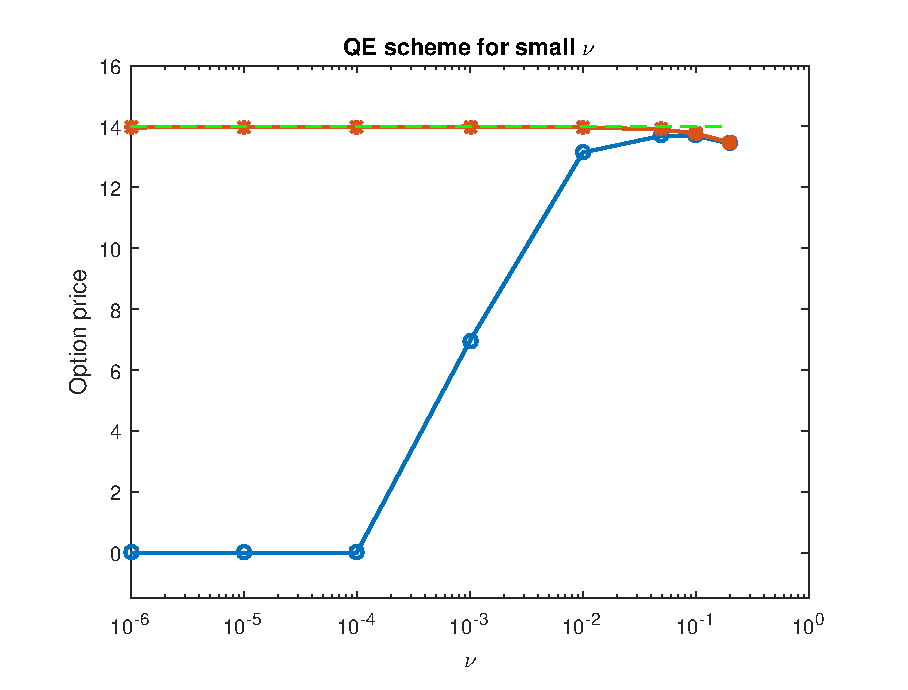
\includegraphics[width=0.55\textwidth]{FigureIn2_3_1.eps}
\caption{European call option price calculate by the QE scheme and our modified QE scheme for an initial price of $\$80$, a strike price of $\$100$, zero interest rate, $T=2$, $\kappa=1$, $\rho=-0.3$, $\theta=0.09$, $V_0=0.36$ and relative tolerance of 1\%. Stars denote the prices calculated by our modified QE scheme when the relative tolerance of 1\% is met. Circles denote the prices calculated by the original QE scheme. The dashed line denotes the option price calculated by the Black-Scholes formula.}
\end{figure}

We calculate the price of European call options with different values of $\nu$. Neither the QE scheme nor the exact sampling works for small $\nu$. When $\nu$ equals zero and the initial variance $V_0$ does not equal to the long-term variance $\theta$, $V_t$ is deterministic and changes over time. We set the variance in the Black-Scholes formula to be the same as the long-term variance $\theta$ and the correct option price should be close to this price when $\nu$ is small. However, the original QE scheme gives zero option price when $\nu$ equals zero and prices close to zero when $\nu$ is close to zero. It is clear from Figure 3.1 that the original QE scheme deviates from the prices calculated by the Black-Scholes model and our modified QE scheme when $\nu$ is smaller than approximately 0.05.

\subsection{Finding a $\gamma$ that is accurate for the approximation of the time integral of V}\label{se:findGamma}

From \eqref{lnX} and \eqref{approxIntV}, the Broadie-Kaya scheme in integral form is written as
\begin{equation}\label{eq:InX_intV}
\begin{split}
    \text{ln}X_{t+\Delta}=&\text{ln}X_t+\frac{\rho}{\nu}(V_{t+\Delta}-V_t-\kappa\theta\Delta)+\bigg(\frac{\kappa\rho}{\nu}-\frac{1}{2}\bigg)\int_{t}^{t+\Delta} V_u du\\
    &+\sqrt{(1-\rho^2)\int_{t}^{t+\Delta}V_u\,\d u}\cdot Z.
\end{split}
\end{equation}

We need to approximate the time-integral of $V$. Rather than simply setting $\gamma=1/2$, we want to find the value of $\gamma$ that makes \eqref{approx_du} exact for $\nu=0$ and show that the error for the approximation of  $\int_{t}^{t+\Delta} V_u du$ is of order $o(\nu\Delta)$. The factor of $\nu$ in the error will then cancel the factor of $1/\nu$ in \eqref{eq:InX_intV}. So, the simulation will be accurate when $\nu$ is close to $0$.

When $\nu=0$, the stochastic partial differential equation of \eqref{eq2} becomes deterministic and has the solution
\begin{equation}\label{V nu=0}
  V_t=\theta + (V_0-\theta)e^{-\kappa t}.
\end{equation}

%Denote $C=V(0)-\theta$,then $V(t)-\theta= Ce^{-\kappa t}$.\\
%\begin{equation}\label{V C}
%  V(t)-\theta= Ce^{-\kappa t}
%\end{equation}
Then, we have
\begin{equation}\label{int V}
  \begin{split}
    \int_{t}^{t+\Delta}V_u\,\d u&=\int_{t}^{t+\Delta}(V_0-\theta)e^{-\kappa u}\,\d u +\theta\Delta\\
    &=\frac{-(V_0-\theta)e^{-\kappa(t+\Delta)}+(V_0-\theta)e^{-\kappa t}}{\kappa}+\theta\Delta\\
    %&=\frac{V(t)-\theta-V(t+\Delta)+\theta}{\kappa}+\theta\Delta.
  \end{split}
\end{equation}
%We want find a expression of $\theta$ written in terms of $V(t)$ and $V(t+\Delta)$.\\
Setting $t=t+\Delta$ in \eqref{V nu=0} provides us an expression for $\theta$ as% and multiply $e^{\kappa\Delta}$ on both sides, we have
%\begin{equation*}
%  V(t+\Delta)-\theta = Ce^{-\kappa(t+\Delta)}
%\end{equation*}
%Multiply $e^{\kappa\Delta}$ on both sides,
%\begin{equation*}
%  e^{\kappa\Delta}(V(t+\Delta)-\theta)=Ce^{-\kappa  t}
%\end{equation*}
%Combine with $V(t)-\theta= Ce^{-\kappa t}$, we have the expression of $\theta$ as
\begin{equation*}
%  \begin{split}
%    & e^{\kappa\Delta}V(t+\Delta)-V(t)+\theta(1-e^{\kappa\Delta})=0 \\
%    & \theta=\frac{V(t)-e^{\kappa\Delta}V(t+\Delta)}{1-e^{\kappa\Delta}}
%  \end{split}
\theta=\frac{V_t-e^{\kappa\Delta}V_{t+\Delta}}{1-e^{\kappa\Delta}}
\end{equation*}
By substituting the above expression of $\theta$ into \eqref{int V}, we obtain
\begin{equation*}
  \begin{split}
    \int_{t}^{t+\Delta}V_u\,\d u &= \frac{V_t-V_{t+\Delta}}{\kappa}+\Delta\frac{V_t-e^{\kappa\Delta}V_{t+\Delta}}{1-e^{\kappa\Delta}}  \\
    %&=\frac{V_t(1-e^{\kappa\Delta}+\kappa\Delta)-V_{t+\Delta}(1-e^{\kappa\Delta}+\kappa\Delta e^{\kappa\Delta})}{\kappa(1-e^{\kappa\Delta})} \\
     %&=\Delta[\gamma_1 V(t)+\gamma_2 V(t+\Delta)]
     &=\Delta[\gamma V_t+(1-\gamma) V_{t+\Delta}],
  \end{split}
\end{equation*}
where
\begin{equation}\label{eq:gamma}
  \gamma = \frac{1-e^{\kappa\Delta}+\kappa\Delta}{\kappa\Delta(1-e^{\kappa\Delta})},\quad 0\leq\gamma\leq1.
\end{equation}

As $\kappa\Delta\rightarrow 0$, $\gamma\rightarrow\frac{1}{2} $.
When $\kappa\Delta$ goes to zero, our scheme becomes the Trapezoidal rule.

We apply the value of $\gamma$ in \eqref{eq:gamma} for all values of $\nu$ to approximate the integral $\int_{t}^{t+\Delta}V_u \,\d u$ and
\begin{equation*}
  \int_{t}^{t+\Delta}V_u\,\d u = \Delta[\gamma V_t+(1-\gamma) V_{t+\Delta}] + O(\nu\Delta^{1.5}).
\end{equation*}
We want to show the error of our approximation for $ \int_{t}^{t+\Delta}V_u\,\d u$ is $o(\nu\Delta)$. 
First, recall the process
\begin{equation*}
  \,\d V_t = \kappa(\theta-V_t)\,\d t +\nu\sqrt{V_t}\,\d W_t\text{,} \quad V_0 \text{ given},
\end{equation*}
defined in \eqref{eq2}. It is not easy to prove directly from process V. So, we define a new process U and let $U_t$ satisfy a similar stochastic differential equation:
\begin{equation*}
  \,\d U_t = -\kappa U_t\,\d t + \nu\sqrt{V_t}\,\d W_t\text{,} \quad U_0 = 0.\numberthis\label{appeqnV_t}
\end{equation*}
Let $Y_t=V_t-U_t$, and note that $Y_t$ satisfies a differential equation:
\begin{equation*}
  %\d (V_t-U_t) = \kappa(\theta-(V_t-U_t))\d t .
  \d Y_t = \kappa(\theta-Y_t)\,\d t, \quad Y_0 = V_0.
\end{equation*}
Moreover, $Y_t=V_t$ when $\nu = 0$. So, we apply similar deduction to $Y_t$ as in Section \ref{se:findGamma}:
%\d Y_t &=\kappa(\theta-Y_t)\d t\\
%\frac{\d Y_t}{\theta-Y_t} &=\kappa \d t\\
%%-\ln(\theta-Y_t) &=\kappa t+C_1\\
\begin{align*}
   \int^{t+\Delta}_t Y_u\,\d u %& =\theta\Delta+(Y_0-\theta)\int^{t+\Delta}_t e^{-\kappa u}\,\d u \\
    %& =\theta\Delta+\frac{(Y_0-\theta)e^{-\kappa t}-(Y_0-\theta)e^{-\kappa (t+\Delta)}}{\kappa}\\
    &= \Delta[\gamma Y_t+(1-\gamma)Y_{t+\Delta}],
\end{align*}
where $\gamma = (1-e^{\kappa\Delta}+\kappa\Delta)\big/\kappa\Delta(1-e^{\kappa\Delta})$.
%\begin{equation*}
% \int_{t}^{t+\Delta}(V_u-U_u)\,\d u =\int^{t+\Delta}_t Y_u\,\d u= \Delta(\gamma_1Y_t+(1-\gamma_1)Y_{t+\Delta})
%\end{equation*}
%where $\gamma_1$ and $(1-\gamma)$ are the same as in Section 3.1.1.\\
Now we have the integral of $V_t$ written in terms of $V$ and $U$ as follows:
\begin{align*}
   \int_{t}^{t+\Delta}V_u\,\d u &= \int_{t}^{t+\Delta}(Y_u+U_u)\,\d u\\
   %&=\Delta[\gamma Y_t+(1-\gamma )Y_{t+\Delta}]+\int_{t}^{t+\Delta}U_u\,\d u\\
   &=\Delta[\gamma  V_t+(1-\gamma ) V_{t+\Delta}]-\bigg\{\Delta[\gamma  U_t+(1-\gamma ) U_{t+\Delta}]-\int_{t}^{t+\Delta}U_u\,\d u\bigg\}.\numberthis\label{intV_U}
\end{align*}
Our problem is to show that the error in approximating $\int_{t}^{t+\Delta}U_u\,\d u$ by\\ $\Delta[\gamma_1 U_t+(1-\gamma_1) U_{t+\Delta}]$ is $o(\nu\Delta)$.

We can write the solution of $U_t$ as
%\begin{equation*}
%  \begin{split}
%     \d e^{\kappa t}U_t & = \kappa e^{\kappa t}U_t\,\d t + e^{\kappa t}\,\d U_t \\
%       & = \kappa e^{\kappa t}U_t \,\d t +e^{\kappa t}(-\kappa U_t\,\d t+\nu\sqrt{V_t}\,\d W_t) \\
%       &= \nu e^{\kappa t}\sqrt{V_t}\,\d W_t
%  \end{split}
%\end{equation*}
%Integrate on both sides,
\begin{align*}
  %f_t & = \nu\int_{0}^{t}e^{\kappa s}\sqrt{V_s}\,\d W_s \\
  U_t & = \nu e^{-\kappa t}\int_{0}^{t}e^{\kappa s}\sqrt{V_s}\,\d W_s.
\end{align*}
Now we rewrite the integral of $U_t$ by using integration by parts twice and \eqref{appeqnV_t}:
\begin{align*}
  \int_{t}^{t+\Delta}U_u\,\d u %& = \int_{t}^{t+\Delta}U_u\,\d (u-t-\Delta\gamma_1) \\
   & = U_u(u-t-\Delta\gamma)\big|_t^{t+\Delta}-\int_{t}^{t+\Delta}(u-t-\Delta\gamma)\,\d U_u \\
   %& = U_u(u-t-\Delta\gamma_1)|_t^{t+\Delta}-\int_{t}^{t+\Delta}(u-t-\Delta\gamma_1)(-\kappa U_u\,\d u +\nu\sqrt{V_u}\,\d W_u)\\
%\end{align*}
%Let $A=-t-\Delta\gamma_1$,
%\begin{align*}
 % \int_{t}^{t+\Delta}U_u\,\d u
 %& = U_{t+\Delta}(t+\Delta-t-\Delta\gamma_1)-U_{t}(-\Delta\gamma_1)-\int_{t}^{t+\Delta}(u-t-\Delta\gamma_1)(-\kappa U_u)\,\d u\\
 % & -\int_{t}^{t+\Delta}(u-t-\Delta\gamma_1)\nu\sqrt{V_u}\,\d W_u \\
%& = \Delta\big[\gamma U_t+(1-\gamma ) U_{t+\Delta}\big]+\int_{t}^{t+\Delta}(u-t-\Delta\gamma )\kappa U_u\,\d u\\
%   &\quad\quad-\nu\int_{t}^{t+\Delta}(u-t-\Delta\gamma )\sqrt{V_u}\,\d W_u\\%\numberthis\label{appeqnU_t}
%   %& = \Delta\big(\gamma U_t+(1-\gamma ) U_{t+\Delta}\big)+\int_{t}^{t+\Delta}\kappa U_u\,\d \big(\frac{(u-t-\Delta\gamma )^2}{2}-\frac{\Delta^2\gamma ^2}{2}\big)\\
%   %&\quad\quad-\nu\int_{t}^{t+\Delta}(u-t-\Delta\gamma )\sqrt{V_u}\,\d W_u\\
%   & = \Delta\big[\gamma U_t+(1-\gamma ) U_{t+\Delta}\big]+\frac{1}{2}\kappa U_{u}\big[{(u-t-\Delta\gamma )^2}-{\Delta^2\gamma ^2}\big]\big|_t^{t+\Delta}\\
%   &\quad\quad- \int_{t}^{t+\Delta}\frac{1}{2}\big[(u-t-\Delta\gamma )^2-\Delta^2\gamma ^2\big] \kappa\,\d U_u\\
%   &\quad\quad-\nu\int_{t}^{t+\Delta}(u-t-\Delta\gamma )\sqrt{V_u}\,\d W_u\\
   & = \Delta\big[\gamma U_t+(1-\gamma ) U_{t+\Delta}\big]+\kappa U_{t+\Delta}\Delta^2\bigg(\frac{1}{2}-\gamma \bigg)\\
   &\quad\quad+\int_{t}^{t+\Delta}(u-t)\bigg[\frac{(u-t)}{2}-\Delta\gamma \bigg]\kappa^2U_u\,\d u\\
   &\quad\quad-\nu\int_{t}^{t+\Delta}h(u)\sqrt{V_u}\,\d W_u,\numberthis\label{appeqnU_t}
\end{align*}
where $h(u) =\kappa(u-t)\big[{(u-t)}/{2}-\Delta\gamma \big]+u-t-\Delta\gamma$.
%\begin{align*}
%   \int_{t}^{t+\Delta}(u-t-\Delta\gamma_1)(-\kappa U_u)\,\d u & = \int_{t}^{t+\Delta}\frac{1}{2}(-\kappa U_u)\,\d (u-t-\Delta\gamma_1)^2\\
%   & = -\int_{t}^{t+\Delta}\kappa U_u\,\d \big(\frac{(u-t-\Delta\gamma_1)^2}{2}-\frac{\Delta^2\gamma_1^2}{2}\big)\\
%   & = -\kappa U_{u}\big(\frac{(u-t-\Delta\gamma_1)^2}{2}-\frac{\Delta^2\gamma_1^2}{2}\big)\big|_t^{t+\Delta}+\int_{t}^{t+\Delta}\big(\frac{(u-t-\Delta\gamma_1)^2}{2}-\frac{\Delta^2\gamma_1^2}{2}\big)\kappa \,\d U_u\\
%   %& = -\kappa U_{t+\Delta}\big(\frac{\Delta^2(1-\gamma_1)^2}{2}-\frac{\Delta^2\gamma_1^2}{2}\big)+\kappa U_{t}\big(\frac{\Delta^2\gamma_1^2}{2}-\frac{\Delta^2\gamma_1^2}{2}\big)\\
%   %& + \int_{t}^{t+\Delta}\big(\frac{(u-t-\Delta\gamma_1)^2}{2}-\frac{\Delta^2\gamma_1^2}{2}\big)\kappa\,\d U_u\\
%%\end{align*}
%%Let $B=-\frac{\Delta^2\gamma_1^2}{2}$,
%%\begin{align*}
%   %\int_{t}^{t+\Delta}(u-t-\Delta\gamma_1)(-\kappa U_u)\,\d u
%   & = \kappa U_{t+\Delta}\big(\frac{(1-\gamma_1)^2-\gamma_1^2}{2}\Delta^2\big)+ \int_{t}^{t+\Delta}\big(\frac{(u-t-\Delta\gamma_1)^2}{2}-\frac{\Delta^2\gamma_1^2}{2}\big)\kappa \,\d U_u\\
%   & = -\kappa U_{t+\Delta}\Delta^2\bigg(\frac{1}{2}-\gamma_1\bigg)+\int_{t}^{t+\Delta}\bigg(\frac{(u-t)^2}{2}-(u-t)\Delta\gamma_1\bigg)\kappa\,\d U_u\\
%   %& = O(\nu\Delta^2)+\int_{t}^{t+\Delta}\bigg(\frac{(u-t)^2}{2}-(u-t)\Delta\gamma_1\bigg)\kappa\,\d U_u\\
%   & = O(\nu\Delta^2)+\int_{t}^{t+\Delta}\bigg(\frac{(u-t)^2}{2}-(u-t)\Delta\gamma_1\bigg)\kappa \,\d (-\kappa U_u\,\d u + \nu\sqrt{V_u}\,\d W_u)\\
%   & = O(\nu\Delta^2)-\int_{t}^{t+\Delta}\bigg(\frac{(u-t)^2}{2}-(u-t)\Delta\gamma_1\bigg)\kappa^2U_u\,\d u\\
%   & + \int_{t}^{t+\Delta}\bigg(\frac{(u-t)^2}{2}-(u-t)\Delta\gamma_1\bigg)\kappa\nu\sqrt{V_u}\,\d W_u\\
%   & = O(\nu\Delta^2)
%\end{align*}
Since $U_t=O(\nu)$, it is easy to see that the second term in \eqref{appeqnU_t} is $O(\nu\Delta^2)$. By H\"older's inequality, the third term of \eqref{appeqnU_t} is
\begin{align*}
   & \int_{t}^{t+\Delta}\bigg(\frac{(u-t)^2}{2}-(u-t)\Delta\gamma \bigg)\kappa^2U_u\,\d u \\
   &\quad\quad\leq\,\, \Delta\gamma \kappa^2\sqrt{\int_{t}^{t+\Delta}\bigg(\frac{(u-t)^2}{2}-(u-t)\Delta\gamma \bigg)^2\,\d u\int_{t}^{t+\Delta}U_u^2\,\d u}\\
   &\quad\quad = \,\,O(\nu\Delta^3).
\end{align*}
Now we want to show that $$I =\nu\int_{t}^{t+\Delta}h(u)\sqrt{V_u}\,\d W_u=O(\nu\Delta^{1.5}).$$
Since $V_t$ is a Cox-Ingersoll-Ross process, we know that its expectation given $V_0$ is $\mathbb{E}(V_t)=V_0 e^{-\kappa u}+\theta(1-e^{-\kappa u})$ \cite{Dufresne2001}, which is O(1). Also, since $\max\limits_{t\leq u\leq t+\Delta}|h(u)|=O(\Delta)$,
\begin{equation*}
\begin{split}
\mathbb{E}\bigg(\nu^2 \int_{t}^{t+\Delta}[h(u)]^2 V_u\,\d u\bigg)  &=\nu^2\int_{t}^{t+\Delta}[h(u)]^2 \mathbb{E}(V_u)\,\d u\\
&=\nu^2\int_{t}^{t+\Delta}O(\Delta^2)\,\d u\\
&=O(\nu^2\Delta^3)\\
&<\infty,
\end{split}
\end{equation*}
we have $I\in\cL^2$ and $I$ is an It\^o integral.
By Theorem 4.7 of \cite{Klebaner2005}, It\^o integral $I$ is a continuous zero mean square integrable martingale.   Thus, by the It\^o isometry,
\begin{align*}
 %\mathbb{E}(I)&= 0\\
  \text{Var}(I)&= \mathbb{E}(I^2)-[\mathbb{E}(I)]^2 \\
  &= \mathbb{E}\bigg(\nu^2 \int_{t}^{t+\Delta}[h(u)]^2 V_u\,\d u\bigg)\\
  %&=\nu^2\int_{t}^{t+\Delta}[h(u)]^2 \mathbb{E}(V_u)\,\d u\\
 % &=\nu^2\int_{t}^{t+\Delta}\big(\frac{(u-t)^2}{2}-\Delta\gamma_1(u-t)\big)^2\kappa^2 \mathbb{E}(V_u)\,\d u\\
%  &=\kappa^2\nu^2\bigg[\int_{t}^{t+\Delta}\frac{1}{20} (V_0 e^{-\kappa u}+\theta(1-e^{-\kappa u})) \,\d (u-t)^5\\
%  &-\int_{t}^{t+\Delta}\frac{1}{4}\Delta\gamma_1 (V_0 e^{-\kappa u}+\theta(1-e^{-\kappa u}))\,\d (u-t)^4\\
%  &+\int_{t}^{t+\Delta}\frac{\Delta^2}{3}\gamma_1^2(V_0 e^{-\kappa u}+\theta(1-e^{-\kappa u})) \,\d(u-t)^3\bigg]\\
%  &=\kappa^2\nu^2 \Delta^5\bigg(\frac{1}{20}(V_0 e^{-\kappa (\xi^\frac{1}{5}+t)}+\theta(1-e^{-\kappa (\xi^\frac{1}{5}+t)})-\frac{1}{4}\gamma_1(V_0 e^{-\kappa (\xi^\frac{1}{4}+t)}+\theta(1-e^{-\kappa (\xi^\frac{1}{4}+t)})\\
%  &+\frac{1}{3}\gamma_1^2(V_0 e^{-\kappa (\xi^\frac{1}{3}+t)}+\theta(1-e^{-\kappa(\xi^\frac{1}{3}+t)}))\bigg)
%&=\nu^2\int_{t}^{t+\Delta}O(\Delta^2)\,\d u\\
&=O(\nu^2\Delta^3).
\end{align*}
%where $\xi\in[t,t+\Delta]$.\\
%Therefore, I is a normal random variable with mean zero and variance of order $O(\nu^2\Delta^5)$. I is of order $O(\nu\Delta^{2.5})$.\\
%Similarly, for the third term of Equation \ref{appeqnU_t}, Ito integral $\int_{t}^{t+\Delta}(u-t-\Delta\gamma_1)\nu\sqrt{V_u}\,\d W_u$ is also a normal distributed random variable with mean zero and variance of order $O(\nu^2\Delta^{3})$.
So, $I$ is a normal distributed random variable with mean zero and variance of order $O(\nu^2\Delta^{3})$. The It\^o integral $I$ is $O(\nu\Delta^{1.5})$.
This implies that
\begin{equation*}
   \int_{t}^{t+\Delta}U_u\,\d u = \Delta\big(\gamma U_t+(1-\gamma) U_{t+\Delta}\big)+O(\nu\Delta^{1.5})
\end{equation*}
in distribution, and so by \eqref{intV_U}
\begin{equation*}
    \int_{t}^{t+\Delta}V_u\,\d u=\Delta\big(\gamma V_t+(1-\gamma) V_{t+\Delta}\big)+O(\nu\Delta^{1.5}),
\end{equation*}
also in distribution.
%\begin{align*}
%  \gamma_1 &= \frac{1-e^{\kappa\Delta}+\kappa\Delta}{\kappa\Delta(1-e^{\kappa\Delta})} &
%  \gamma_2 &= -\frac{1-e^{\kappa\Delta}+\kappa\Delta e^{\kappa\Delta}}{\kappa\Delta(1-e^{\kappa\Delta})}
%\end{align*}
%$\gamma_1 =
%$\gamma = \frac{1-e^{\kappa\Delta}+\kappa\Delta}{\kappa\Delta(1-e^{\kappa\Delta})}$,
%$\gamma_2 = -\frac{1-e^{\kappa\Delta}+\kappa\Delta e^{\kappa\Delta}}{\kappa\Delta(1-e^{\kappa\Delta})}$.
%We know $\gamma_1\geq 0$ and $\gamma_2\geq 0$.\\
%$\gamma\geq 0$.
%As $\kappa\Delta\rightarrow 0$, $\gamma\rightarrow\frac{\frac{1}{2}(\kappa\Delta)^2}{\kappa\Delta}=\frac{1}{2} $.\\
%\begin{align*}
% \gamma_1 &\rightarrow\frac{\frac{1}{2}(\kappa\Delta)^2}{\kappa\Delta}=\frac{1}{2} \\
%  \gamma_2 &\rightarrow\frac{-(1+\kappa\Delta+\frac{1}{2}(\kappa\Delta)^2)(1-\kappa\Delta)+1}{\kappa\Delta(\kappa\Delta)}
%  \rightarrow\frac{-(1-(\kappa\Delta)^2)-\frac{1}{2}(\kappa\Delta)^2+\frac{1}{2}(\kappa\Delta)^3+1}{(\kappa\Delta)^2}\rightarrow\frac{1}{2}
%\end{align*}
%When $\kappa\Delta$ goes to zero, our scheme just like the Euler scheme.\\
%For $\nu\neq 0$, we approximate the integral $\int_{t}^{t+\Delta}V(u)\d u$ as follow:
%\begin{equation*}
%  \int_{t}^{t+\Delta}V(u)\d u = \Delta[\gamma V(t)+(1-\gamma) V(t+\Delta)] + O(\nu\Delta^{1.5}).
%\end{equation*}
%See the proof of the error order of this approximation in ~\ref{sec:AppendixA}.
\subsection{Change of variables to avoid overflow}
%We want to do change of variable of $s^2, m, \psi, b^{-2}, a, b, K_0,K_1,K_2, K_3,$ and $ K_4$ in a way that $\nu$ becomes multiplier rather than divisor.\\
Another problem with the formula \eqref{eq:InX_intV} is that $\nu$ appears in the denominator. This may lead to numerical error when $\nu$ is small. To avoid this error we make a change of variables of $s^2, \psi, b^{-2}, a, b, $ $K_0,K_1,K_2, K_3,$ and $ K_4$.
We first make a change of variables in the QE scheme
%, we do change of variables. As we see, new variables $\tilde{s}^2, \tilde{m}$ and $\tilde{\psi}$ are free of $\nu$.
%\begin{align*}
%s^2&=\nu^2\tilde{s}^2 & \tilde{s}^2 &=\frac{\hat{V}(t)e^{-\kappa\Delta}}{\kappa}\bigg(1-e^{-\kappa\Delta}\bigg)+\frac{\theta}{2\kappa}\bigg(1-e^{-\kappa\Delta}\bigg)^2, \\
%m&=\tilde{m} & \tilde{m} &=\Theta + \hat{V}(t)e^{-\kappa\Delta} \\
%  \psi&=\tilde{\psi}\nu^2, & \tilde{\psi}&=\bigg(\frac{\frac{\hat{V}(t)e^{-\kappa\Delta}}{\kappa}(1-e^{-\kappa\Delta})+\frac{\theta}{2\kappa}(1-e^{-\kappa\Delta})^2}{(\theta+(\hat{V}(t)-\theta)e^{-\kappa\Delta})^2}\bigg)\\
%  b^{-2}&=\nu^2\tilde{b}^{-2}, & \tilde{b}^{-2}&=\frac{\tilde{\psi}}{2\sqrt{1-\frac{\tilde{\psi}\nu^2}{2}}\bigg(1+\sqrt{1-\frac{\tilde{\psi}\nu^2}{2}}\bigg)} \\
%  a&=\tilde{a}\nu^2, & \tilde{a}&=\frac{m\tilde{b}^{-2}}{1+\nu^2\tilde{b}^{-2}}
%\end{align*}
%\begin{align*}
%s^2&=\nu^2\tilde{s}^2={\nu}^2\bigg(\frac{\hat{V}(t)e^{-\kappa\Delta}}{\kappa}\big(1-e^{-\kappa\Delta}\big)+\frac{\theta}{2\kappa}\big(1-e^{-\kappa\Delta}\big)^2\bigg),
%\quad m=\tilde{m}=\theta + \hat{V}(t)e^{-\kappa\Delta}, \\
%  \psi&=\nu^2\tilde{\psi}=\nu^2\bigg[\frac{\frac{\hat{V}(t)e^{-\kappa\Delta}}{\kappa}(1-e^{-\kappa\Delta})+\frac{\theta}{2\kappa}(1-e^{-\kappa\Delta})^2}{\big(\theta+(\hat{V}(t)-\theta)e^{-\kappa\Delta}\big)^2}\bigg],\\
%b^{-2}&=\nu^2\tilde{b}^{-2}=\nu^2\frac{\tilde{\psi}}{2\sqrt{1-\frac{\tilde{\psi}\nu^2}{2}}\bigg(1+\sqrt{1-\frac{\tilde{\psi}\nu^2}{2}}\bigg)} ,\quad
%a=\nu^2\tilde{a}=\nu^2\frac{m\tilde{b}^{-2}}{1+\nu^2\tilde{b}^{-2}}.
%\end{align*}

\begin{align*}
\tilde{s}^2&={\nu}^{-2}s=\frac{\hat{V}_t e^{-\kappa\Delta}}{\kappa}\big(1-e^{-\kappa\Delta}\big)+\frac{\theta}{2\kappa}\big(1-e^{-\kappa\Delta}\big)^2,
%\quad m=\tilde{m}=\theta + \hat{V}_te^{-\kappa\Delta}, \\
\\
\tilde{\psi}&= \nu^{-2}\psi=\frac{\frac{\hat{V}_te^{-\kappa\Delta}}{\kappa}(1-e^{-\kappa\Delta})+\frac{\theta}{2\kappa}(1-e^{-\kappa\Delta})^2}{\big(\theta+(\hat{V}_t-\theta)e^{-\kappa\Delta}\big)^2},\\
\tilde{b}^{-2}&=\nu^{-2}b^{-2}=\frac{\tilde{\psi}}{2\sqrt{1-\frac{\tilde{\psi}\nu^2}{2}}\bigg(1+\sqrt{1-\frac{\tilde{\psi}\nu^2}{2}}\bigg)} ,\\
\tilde{a}&=\nu^{-2}a=\frac{m\tilde{b}^{-2}}{1+\nu^2\tilde{b}^{-2}}.
\end{align*}

%Similarly, for parameters in Broadie-Kaya discretization scheme, we have

As we see, new variables $\tilde{s}^2$ and $\tilde{\psi}$ are free of $\nu$. Moreover, as $\nu\rightarrow0$, $\tilde{a}$ and $\tilde{b}$ have finite limits. After making the change of variables, when $\nu$ goes to $0$, our new variables have finite limits.
Now we use new variables that we defined to calculate $\hat{X}$. Recall \eqref{eq3}:

\begin{equation*}
  \text{ln}\hat{X}_{t+\Delta}=\text{ln}\hat{X}_t+K_0+K_1\hat{V}_t+K_2\hat{V}_{t+\Delta}+\sqrt{K_3\hat{V}_{t}+K_4\hat{V}_{t+\Delta}}\cdot Z.
\end{equation*}

Observe the expression of parameters we discussed in Section \ref{se:B-K}, the terms including $\nu^{-1}$ will cause overflow when $\nu$ is close or equal to zero. We want to define a new variable of stochastic volatility process $V$ in a way that there is no $\nu^{-1}$ in our modified discretization scheme.

Define $\tilde{V}_t=\hat{V}_t-\theta$ and write $\hat{V}_{t+\Delta}$ in terms of new variables:
\begin{equation*}
\begin{split}
\hat{V}_{t+\Delta}%&=\frac{\tilde{m}\tilde{b}^{-2}}{1+\nu^2\tilde{b}^{-2}}(\tilde{b}+\nu Z_V)^2\\
%&=\frac{\tilde{m}}{1+\nu^2\tilde{b}^{-2}}(1+\nu\tilde{b}^{-1}Z_V)^2\\
&=\frac{\theta+\tilde{V}_te^{-\kappa\Delta}}{1+\nu^2\tilde{b}^{-2}}(1+\nu\tilde{b}^{-1}Z_V)^2.
\end{split}
\end{equation*}

Then, we have the expression of $\tilde{V}_{t+\Delta}$ as
\begin{equation*}
\begin{split}
\tilde{V}_{t+\Delta}%&=\hat{V}(t+\Delta)-\theta\\
%&=\frac{\theta+\tilde{V}(t)e^{-\kappa\Delta}}{1+\nu^2\tilde{b}^{-2}}(1+\nu\tilde{b}^{-1}Z_V)^2-\theta\\
%&=\frac{\theta[(1+\nu\tilde{b}^{-1}Z_V)^2-(1+\nu^2\tilde{b}^{-2})]+\tilde{V}(t)e^{-\kappa\Delta}(1+\nu\tilde{b}^{-1}Z_V)^2}{1+\nu^2\tilde{b}^{-2}}\\
%&=\frac{\theta\nu[2\tilde{b}^{-1}Z_V+\nu(\tilde{b}^{-2}Z_V^2-\tilde{b}^{-2})]+\tilde{V}(t)e^{-\kappa\Delta}(1+\nu\tilde{b}^{-1}Z_V)^2}{1+\nu^2\tilde{b}^{-2}}\\
&=\frac{\theta\nu[2\tilde{b}^{-1}Z_V+\nu\tilde{b}^{-2}(Z_V^2-1)]+\tilde{V}_te^{-\kappa\Delta}(1+\nu\tilde{b}^{-1}Z_V)^2}{1+\nu^2\tilde{b}^{-2}}.
\end{split}
\end{equation*}

Define $ \mathring{V}_{t+\Delta}=(\tilde{V}_{t+\Delta}-\tilde{V}_te^{-\kappa\Delta})\big/{\nu }$,

\begin{equation*}
\begin{split}
\mathring{V}_{t+\Delta}
%&=\frac{1}{\nu}[\tilde{V}(t+\Delta)-\tilde{V}(t)e^{-\kappa\Delta}]\\
%&=\frac{1}{\nu}[\hat{V}_{t+\Delta}-(\theta+\tilde{V}_te^{-\kappa\Delta})]\\
%&=\frac{\theta+\tilde{V}(t)e^{-\kappa\Delta}}{\nu}\bigg[\frac{(1+\nu\tilde{b}^{-1}Z_V)^2}{1+\nu^2b^{-2}}-1\bigg]\\
&=(\theta+\tilde{V}_te^{-\kappa\Delta})\bigg[\frac{2\tilde{b}^{-1}Z_V}{1+\nu^2\tilde{b}^{-2}}+\nu\frac{\tilde{b}^{-2}(Z_V^2-1)}{1+\nu^2\tilde{b}^{-2}}\bigg].
\end{split}
\end{equation*}

In order to calculate $\text{ln}\hat{X}$, we note that
\begin{equation*}
\begin{split}
&\gamma\tilde{V}_{t}+(1-\gamma)\tilde{V}_{t+\Delta}
%=& (\gamma_1+\gamma_2e^{-\kappa\Delta})\tilde{V}(t)+\gamma_2\nu\mathring{V}(t+\Delta)\\
=%&
\frac{1-e^{-\kappa\Delta}}{\kappa\Delta}\tilde{V}_t+(1-\gamma)\nu\mathring{V}_{t+\Delta}.\\
\end{split}
\end{equation*}

Substituting the above equation into the following equation:
\begin{equation}\label{QEK0K1K2}
\begin{split}
&K_0+K_1\hat{V}_t+K_2\hat{V}_{t+\Delta}
%&\quad\quad=(K_0+\theta K_1+\theta K_2)+K_1\tilde{V}_t+K_2\tilde{V}_{t+\Delta}\\
%=&\frac{\rho\kappa\Delta}{\nu}(-\theta+\gamma_1\theta+\gamma_2\theta)-\frac{\rho\theta}{\nu}+\frac{\rho\theta}{\nu}+\theta\Delta(-\frac{1}{2})(\gamma_1+\gamma_2)\\
%&+\frac{\kappa\Delta\rho}{\nu}(\gamma_1\tilde{V}(t)+\gamma_2\tilde{V}(t+\Delta))-\frac{\Delta}{2}(\gamma_1\tilde{V}(t)+\gamma_2\tilde{V}(t+\Delta))+\frac{\rho}{\nu}(-\tilde{V}(t)+\tilde{V}(t+\Delta))\\
%=&-\theta\frac{\Delta}{2}-\frac{\Delta}{2}(\gamma_1\tilde{V}(t)+\gamma_2\tilde{V}(t+\Delta))+\frac{\rho}{\nu}[(-1+\kappa\Delta\gamma_1)\tilde{V}(t)+(1+\kappa\Delta\gamma_2)\tilde{V}(t+\Delta)]\\
%=&\theta\frac{\Delta}{2}-\frac{\Delta}{2}(\gamma_1\tilde{V}(t)+\gamma_2\tilde{V}(t+\Delta))+\frac{\rho}{\nu}\bigg[\frac{\kappa\Delta e^{\kappa\Delta}}{e^{\kappa\Delta}-1}\tilde{V}(t+\Delta)-\frac{\kappa\Delta}{e^{\kappa\Delta}-1}\tilde{V}(t)\bigg]\\
%=&-\theta\frac{\Delta}{2}-\frac{\Delta}{2}(\gamma_1\tilde{V}(t)+\gamma_2\tilde{V}(t+\Delta))+\frac{\rho}{\nu}\frac{\kappa\Delta e^{\kappa\Delta}}{e^{\kappa\Delta}-1}(\tilde{V}(t+\Delta)-\tilde{V}(t)e^{-\kappa\Delta})\\
%&\quad\quad=-\theta\frac{\Delta}{2}-\frac{\Delta}{2}\big[\gamma\tilde{V}_t+(1-\gamma)\tilde{V}_{t+\Delta}\big]+\frac{\rho\kappa\Delta e^{\kappa\Delta}}{e^{\kappa\Delta}-1}\mathring{V}_{t+\Delta}\\
%=&-\theta\frac{\Delta}{2}-\frac{\Delta}{2}\bigg(\frac{1-e^{-\kappa\Delta}}{\kappa\Delta}\tilde{V}(t)+\gamma_2\nu\mathring{V}(t+\Delta)\bigg)+\frac{\rho\kappa\Delta e^{\kappa\Delta}}{e^{\kappa\Delta}-1}\mathring{V}(t+\Delta)\\
%\quad\quad
=-\theta\frac{\Delta}{2}-\frac{1-e^{-\kappa\Delta}}{2\kappa}\tilde{V}_t-\bigg[\frac{\nu(1-e^{\kappa\Delta}+\kappa\Delta e^{\kappa\Delta})}{2\kappa(1-e^{\kappa\Delta})}+\frac{\rho\kappa\Delta e^{\kappa\Delta}}{1-e^{\kappa\Delta}}\bigg]\mathring{V}_{t+\Delta}.
\end{split}
\end{equation}

Moreover,
\begin{align*}
&K_3\hat{V}_t+K_4\hat{V}_{t+\Delta}
%=&\gamma_1\Delta(1-\rho^2)\hat{V}(t)+\gamma_2\Delta(1-\rho^2)\hat{V}(t+\Delta)\\
%=&\Delta(1-\rho^2)[\gamma_1(\theta+\tilde{V}(t))+\gamma_2(\theta+\tilde{V}(t+\Delta))]\\
%&\quad\quad=\Delta(1-\rho^2)\big[\theta+\gamma\tilde{V}_t+(1-\gamma)\tilde{V}_{t+\Delta}\big]\\
%=&\Delta(1-\rho^2)\big[\theta+\big((\gamma_1+\gamma_2e^{-\kappa\Delta})\tilde{V}(t)+\gamma_2\nu \mathring{V}(t+\Delta)\big)\big]\\
%&\quad\quad
=\Delta(1-\rho^2)\bigg\{\theta+\bigg[\frac{1-e^{-\kappa\Delta}}{\kappa\Delta}\tilde{V}_t+(1-\gamma)\nu \mathring{V}_{t+\Delta}\bigg]\bigg\}.\numberthis\label{QEK3K4}
\end{align*}

Now we can rewrite the discretization scheme.
For the discretization scheme of $X$ when $\nu^2\tilde{\psi} \leq \psi_c $:
\begin{equation}\label{newLnX}
\begin{split}
  \ln\hat{X}_{t+\Delta}=&\ln\hat{X}_t-\theta\frac{\Delta}{2}-\frac{1-e^{-\kappa\Delta}}{2\kappa}\tilde{V}_t-\bigg[\frac{\nu(1-e^{\kappa\Delta}+\kappa\Delta e^{\kappa\Delta})}{2\kappa(1-e^{\kappa\Delta})}+\frac{\rho\kappa\Delta e^{\kappa\Delta}}{1-e^{\kappa\Delta}}\bigg]\mathring{V}_{t+\Delta}\\
  &+\sqrt{\Delta(1-\rho^2)\bigg\{\theta+\bigg[\frac{1-e^{-\kappa\Delta}}{\kappa\Delta}\tilde{V}_t+(1-\gamma)\nu \mathring{V}_{t+\Delta}\bigg]\bigg\}}\cdot Z.
\end{split}
\end{equation}

Since the discretization scheme is inaccurate only when $\nu$ is small, we will only apply our modifications to $\nu^2\tilde{\psi} \leq \psi_c $. For the $\nu^2\tilde{\psi} > \psi_c $ case, the scheme remains unchanged:

\begin{equation}\label{newLnX2}
  \text{ln}\hat{X}_{t+\Delta}=\text{ln}\hat{X}_t+{K}_0+\frac{1}{\nu}{K}_1\hat{V}_t+\frac{1}{\nu}{K}_2\hat{V}_{t+\Delta}+\sqrt{{K}_3\hat{V}_t+{K}_4\hat{V}_{t+\Delta}}\cdot Z.
\end{equation}

%\begin{align*}
%   K_0&=\frac{1}{\nu}\tilde{K}_0 =\frac{1}{\nu}(-\rho\kappa\theta\Delta),&   K_1&=\frac{1}{\nu}\tilde{K_1}=\frac{1}{\nu}\bigg[\rho(\kappa\gamma\Delta-1)-\frac{\nu\gamma\Delta}{2}\bigg],\\  K_2&=\frac{1}{\nu}\tilde{K_2}=\frac{1}{\nu}\bigg[\rho\big(\kappa(1-\gamma)\Delta-1\big)-\frac{\nu(1-\gamma)\Delta}{2}\bigg], &
%   K_3&=\tilde{K}_3=\gamma\Delta(1-\rho^2),\\ K_4&=\tilde{K}_4=(1-\gamma)\Delta(1-\rho^2).
%\end{align*}
%\subsubsection{Change of variables for calculating $\hat{X}$}
%For Eq.\eqref{eq2}, set $\nu=0$, we have
%\begin{equation*}
% \begin{split}
% \text{d}V(t)&=\kappa(\theta-V(t))\,\text{d}t\\
% V(T) &=\theta+(V(t)-\theta)e^{-\kappa(T-t)}
%\end{split}
%\end{equation*}
%After doing change of variables, when $\nu$ goes to $0$, our new variables will be certain numbers rather than go to infinity.\\
%Now we use new variables we defined to calculate $\hat{X}$. Recall Eq.\eqref{eq3}:
%\begin{equation*}
%  \text{ln}\hat{X}(t+\Delta)=\text{ln}\hat{X}(t)+K_0+K_1\hat{V}(t)+K_2\hat{V}(t+\Delta)+\sqrt{K_3\hat{V}(t)+K_4\hat{V}(t+\Delta)}\cdot Z
%\end{equation*}
%Observe the expression of parameters we discussed in section 2.3, the terms including $\frac{1}{\nu}$ will cause unstable of the scheme when $\nu$ is close or equal to zero. We want to define a new variable of stochastic volatility process $V$ in a way that there is no $\frac{1}{\nu}$ in our modified discretization scheme.\\
%Write $\hat{V}(t+\Delta)$ in terms of new variables that we defined before,
%\begin{equation*}
%\begin{split}
%\hat{V}(t+\Delta)%&=\frac{\tilde{m}\tilde{b}^{-2}}{1+\nu^2\tilde{b}^{-2}}(\tilde{b}+\nu Z_V)^2\\
%%&=\frac{\tilde{m}}{1+\nu^2\tilde{b}^{-2}}(1+\nu\tilde{b}^{-1}Z_V)^2\\
%&=\frac{\theta+\tilde{V}(t)e^{-\kappa\Delta}}{1+\nu^2\tilde{b}^{-2}}(1+\nu\tilde{b}^{-1}Z_V)^2
%\end{split}
%\end{equation*}
%Define $\tilde{V}(t)=\hat{V}(t)-\theta$.
%Substitute the above equation into the following equation,
%\begin{equation*}
%\begin{split}
%\tilde{V}(t+\Delta)%&=\hat{V}(t+\Delta)-\theta\\
%%&=\frac{\theta+\tilde{V}(t)e^{-\kappa\Delta}}{1+\nu^2\tilde{b}^{-2}}(1+\nu\tilde{b}^{-1}Z_V)^2-\theta\\
%%&=\frac{\theta[(1+\nu\tilde{b}^{-1}Z_V)^2-(1+\nu^2\tilde{b}^{-2})]+\tilde{V}(t)e^{-\kappa\Delta}(1+\nu\tilde{b}^{-1}Z_V)^2}{1+\nu^2\tilde{b}^{-2}}\\
%%&=\frac{\theta\nu[2\tilde{b}^{-1}Z_V+\nu(\tilde{b}^{-2}Z_V^2-\tilde{b}^{-2})]+\tilde{V}(t)e^{-\kappa\Delta}(1+\nu\tilde{b}^{-1}Z_V)^2}{1+\nu^2\tilde{b}^{-2}}\\
%&=\frac{\theta\nu(2\tilde{b}^{-1}Z_V+\nu\tilde{b}^{-2}(Z_V^2-1))+\tilde{V}e^{-\kappa\Delta}(1+\nu\tilde{b}^{-1}Z_V)^2}{1+\nu^2\tilde{b}^{-2}}
%\end{split}
%\end{equation*}
%Define $\nu \mathring{V}(t+\Delta)=\tilde{V}(t+\Delta)-\tilde{V}(t)e^{-\kappa\Delta}$.\\
%\begin{equation*}
%\begin{split}
%\mathring{V}(t+\Delta)%&=\frac{1}{\nu}[\tilde{V}(t+\Delta)-\tilde{V}(t)e^{-\kappa\Delta}]\\
%&=\frac{1}{\nu}[\hat{V}(t+\Delta)-(\theta+\tilde{V}(t)e^{-\kappa\Delta})]\\
%%&=\frac{\theta+\tilde{V}(t)e^{-\kappa\Delta}}{\nu}\bigg[\frac{(1+\nu\tilde{b}^{-1}Z_V)^2}{1+\nu^2b^{-2}}-1\bigg]\\
%&=(\theta+\tilde{V}(t)e^{-\kappa\Delta})\bigg[\frac{2\tilde{b}^{-1}Z_V}{1+\nu^2\tilde{b}^{-2}}+\nu\frac{\tilde{b}^{-2}(Z_V^2-1)}{1+\nu^2\tilde{b}^{-2}}\bigg]
%\end{split}
%\end{equation*}
%In order to calculate $\text{ln}\hat{X}$,we do the following calculation first.\\
%\begin{equation*}
%\begin{split}
%&\gamma\tilde{V}(t)+(1-\gamma)\tilde{V}(t+\Delta)
%%=& (\gamma_1+\gamma_2e^{-\kappa\Delta})\tilde{V}(t)+\gamma_2\nu\mathring{V}(t+\Delta)\\
%=%&
%\frac{1-e^{-\kappa\Delta}}{\kappa\Delta}\tilde{V}(t)+(1-\gamma)\nu\mathring{V}(t+\Delta).\\
%\end{split}
%\end{equation*}
%Substituting the above equation into the following equations, we get
%\begin{equation}\label{QEK0K1K2}
%\begin{split}
%&K_0+K_1\hat{V}(t)+K_2\hat{V}(t+\Delta)\\
%=&(K_0+\theta K_1+\theta K_2)+K_1\tilde{V}(t)+K_2\tilde{V}(t+\Delta)\\
%%=&\frac{\rho\kappa\Delta}{\nu}(-\theta+\gamma_1\theta+\gamma_2\theta)-\frac{\rho\theta}{\nu}+\frac{\rho\theta}{\nu}+\theta\Delta(-\frac{1}{2})(\gamma_1+\gamma_2)\\
%%&+\frac{\kappa\Delta\rho}{\nu}(\gamma_1\tilde{V}(t)+\gamma_2\tilde{V}(t+\Delta))-\frac{\Delta}{2}(\gamma_1\tilde{V}(t)+\gamma_2\tilde{V}(t+\Delta))+\frac{\rho}{\nu}(-\tilde{V}(t)+\tilde{V}(t+\Delta))\\
%%=&-\theta\frac{\Delta}{2}-\frac{\Delta}{2}(\gamma_1\tilde{V}(t)+\gamma_2\tilde{V}(t+\Delta))+\frac{\rho}{\nu}[(-1+\kappa\Delta\gamma_1)\tilde{V}(t)+(1+\kappa\Delta\gamma_2)\tilde{V}(t+\Delta)]\\
%%=&\theta\frac{\Delta}{2}-\frac{\Delta}{2}(\gamma_1\tilde{V}(t)+\gamma_2\tilde{V}(t+\Delta))+\frac{\rho}{\nu}\bigg[\frac{\kappa\Delta e^{\kappa\Delta}}{e^{\kappa\Delta}-1}\tilde{V}(t+\Delta)-\frac{\kappa\Delta}{e^{\kappa\Delta}-1}\tilde{V}(t)\bigg]\\
%%=&-\theta\frac{\Delta}{2}-\frac{\Delta}{2}(\gamma_1\tilde{V}(t)+\gamma_2\tilde{V}(t+\Delta))+\frac{\rho}{\nu}\frac{\kappa\Delta e^{\kappa\Delta}}{e^{\kappa\Delta}-1}(\tilde{V}(t+\Delta)-\tilde{V}(t)e^{-\kappa\Delta})\\
%=&-\theta\frac{\Delta}{2}-\frac{\Delta}{2}\big[\gamma\tilde{V}(t)+(1-\gamma)\tilde{V}(t+\Delta)\big]+\frac{\rho\kappa\Delta e^{\kappa\Delta}}{e^{\kappa\Delta}-1}\mathring{V}(t+\Delta)\\
%%=&-\theta\frac{\Delta}{2}-\frac{\Delta}{2}\bigg(\frac{1-e^{-\kappa\Delta}}{\kappa\Delta}\tilde{V}(t)+\gamma_2\nu\mathring{V}(t+\Delta)\bigg)+\frac{\rho\kappa\Delta e^{\kappa\Delta}}{e^{\kappa\Delta}-1}\mathring{V}(t+\Delta)\\
%=&-\theta\frac{\Delta}{2}-\frac{1-e^{-\kappa\Delta}}{2\kappa}\tilde{V}(t)-\bigg[\frac{\nu(1-e^{\kappa\Delta}+\kappa\Delta e^{\kappa\Delta})}{2\kappa(1-e^{\kappa\Delta})}+\frac{\rho\kappa\Delta e^{\kappa\Delta}}{1-e^{\kappa\Delta}}\bigg]\mathring{V}(t+\Delta)
%\end{split}
%\end{equation}
%Define $\tilde{V}(t)=\hat{V}(t)-\theta$. \\
%If $\nu=0$, we have $$\hat{V}(t+\Delta)-\theta=(\hat{V}(t)-\theta)e^{-\kappa\Delta}$$
%
%i.e. $$\tilde{V}(t+\Delta)=\tilde{V}(t)e^{-\kappa\Delta}$$
%\begin{align*}
%&K_0+K_1\hat{V}(t)+K_2\hat{V}(t+\Delta)=K_0+K_1(\tilde{V}(t)+\theta)+K_2(\tilde{V}(t+\Delta)+\theta)\\
%=&(K_0+K_1\theta+K_2\theta)+K_1\tilde{V}(t)+K_2\tilde{V}(t+\Delta)\\
%=&-\frac{\rho\kappa\Delta}{\nu}(-\theta+\gamma_1\theta+\gamma_2\theta)-\frac{1}{2}\Delta\theta(\gamma_1+\gamma_2)+\frac{\rho}{\nu}(\gamma_1\Delta\kappa-1)\tilde{V}(t)\\
%&-\frac{1}{2}\gamma_1\Delta\tilde{V}(t)+\frac{\rho}{\nu}(\gamma_2\Delta\kappa+1)\tilde{V}(t+\Delta)-\frac{1}{2}\gamma_2\Delta\tilde{V}(t+\Delta)
%\end{align*}
%Moreover,
%\begin{align*}
%&K_3\hat{V}(t)+K_4\hat{V}(t+\Delta)\\
%%=&\gamma_1\Delta(1-\rho^2)\hat{V}(t)+\gamma_2\Delta(1-\rho^2)\hat{V}(t+\Delta)\\
%%=&\Delta(1-\rho^2)[\gamma_1(\theta+\tilde{V}(t))+\gamma_2(\theta+\tilde{V}(t+\Delta))]\\
%=&\Delta(1-\rho^2)\big[\theta+\big(\gamma\tilde{V}(t)+(1-\gamma)\tilde{V}(t+\Delta)\big)\big]\\
%%=&\Delta(1-\rho^2)\big[\theta+\big((\gamma_1+\gamma_2e^{-\kappa\Delta})\tilde{V}(t)+\gamma_2\nu \mathring{V}(t+\Delta)\big)\big]\\
%=&\Delta(1-\rho^2)\bigg[\theta+\bigg(\frac{1-e^{-\kappa\Delta}}{\kappa\Delta}\tilde{V}(t)+(1-\gamma)\nu \mathring{V}(t+\Delta)\bigg)\bigg]\numberthis\label{QEK3K4}
%\end{align*}

%Now we can rewrite the discretization scheme.
%For $X$ when $\nu^2\tilde{\psi} \leq \psi_C $:
%\begin{equation}\label{newLnX}
%\begin{split}
%  \ln\hat{X}(t+\Delta)=&\ln\hat{X}(t)-\theta\frac{\Delta}{2}-\frac{1-e^{-\kappa\Delta}}{2\kappa}\tilde{V}(t)-\bigg(\frac{\nu(1-e^{\kappa\Delta}+\kappa\Delta e^{\kappa\Delta})}{2\kappa(1-e^{\kappa\Delta})}+\frac{\rho\kappa\Delta e^{\kappa\Delta}}{1-e^{\kappa\Delta}}\bigg)\mathring{V}(t+\Delta)\\
%  &+\sqrt{\Delta(1-\rho^2)\bigg[\theta+\bigg(\frac{1-e^{-\kappa\Delta}}{\kappa\Delta}\tilde{V}(t)+(1-\gamma)\nu \mathring{V}(t+\Delta)\bigg)\bigg]}\cdot Z
%\end{split}
%\end{equation}
%For $X$ when $\nu^2\tilde{\psi} > \psi_C $:
%\begin{equation}\label{newLnX2}
%  \text{ln}\hat{X}(t+\Delta)=\text{ln}\hat{X}(t)+\tilde{K}_0+\frac{1}{\nu}\tilde{K}_1\hat{V}(t)+\frac{1}{\nu}\tilde{K}_2\hat{V}(t+\Delta)+\sqrt{\tilde{K}_3\hat{V}(t)+\tilde{K}_4\hat{V}(t+\Delta)}\cdot Z
%\end{equation}
%Since the discretization scheme is unstable only when $\nu$ is very small, for the $\nu^2\tilde{\psi} > \psi_C $ case, the scheme remains unchanged. We just rewrite it in terms of new variables.

\subsection{The modified QE and Broadie-Kaya discretization scheme}
Now we can propose our modified scheme for the Heston model:

%Summary of QE algorithm and the discretization scheme of $X$:
\begin{enumerate}
\item Given $\hat{V}_t$, compute $m$ and $\tilde{s}^2$ from the following equations
\begin{align*}
  m &=\Theta + \tilde{V}_te^{-\kappa\Delta}, \\
  \tilde{s}^2 &=\frac{(\tilde{V}_t+\theta) e^{-\kappa\Delta}}{\kappa}\bigg(1-e^{-\kappa\Delta}\bigg)+\frac{\theta}{2\kappa}\bigg(1-e^{-\kappa\Delta}\bigg)^2.
\end{align*}
\item Compute $\tilde{\psi}=\tilde{s}^2/m^2$.\\
\item Generate two independent normal random variables  $Z_V$ and $Z$ from GAIL.\\
\item If $\nu^2\tilde{\psi}\leq\psi_c$:
\begin{enumerate}
\item Compute $\tilde{a}$ and $\tilde{b}$ from the following equations
\begin{align*}
  \tilde{b}^{-2} & =\frac{\tilde{\psi}}{2\sqrt{1-\frac{1}{2}\tilde{\psi}\nu^2}\bigg(1+\sqrt{1-\frac{1}{2}\tilde{\psi}\nu^2}\bigg)},\\
  \tilde{a} & =\frac{m\tilde{b}^{-2}}{1+\nu^2\tilde{b}^{-2}}.
\end{align*}
%\item Compute $Z_V=\Phi^{-1}(U_V)$
\item Set $\tilde{V}_{t+\Delta}=-\theta + \tilde{a}(\tilde{b}+\nu Z_V)^2.$
\item Compute $\mathring{V}_{t+\Delta}={(\theta+\tilde{V}_te^{-\kappa\Delta})\bigg[\frac{2\tilde{b}^{-1}Z_V}{1+\nu^2\tilde{b}^{-2}}+\frac{\nu\tilde{b}^{-2}(Z_V^2-1)}{1+\nu^2\tilde{b}^{-2}}\bigg]}$.
\item Given $\tilde{V}_t$, $\ln\hat{X}_t$ and the value for $\mathring{V}_{t+\Delta}$, compute $\ln \hat{X}_{t+\Delta}$ from \eqref{newLnX}.
  %\item Given $\tilde{V}_t$, generate $\tilde{V}(t+\Delta)$
  %\item Given $\ln\hat{X}(t)$, $\tilde{V}(t)$ and the value for $\mathring{V}(t+\Delta)$, compute $\ln \hat{X}(t+\Delta)$ from Eq.\eqref{newLnX}
\end{enumerate}
\item Otherwise, if $\nu^2\tilde{\psi}>\psi_c$
\begin{enumerate}
  \item Compute $\beta$ and $p$ according to equations
  \begin{align*}
    p & =\frac{\nu^2\tilde{\psi}-1}{\nu^2\tilde{\psi}+1}\in[0,1), \\
    \beta & =\frac{1-p}{\tilde{m}}=\frac{2}{m(\nu^2\tilde{\psi}+1)}>0.
  \end{align*}
  \item Draw a uniform random number $U_V$.
  \item Set $\tilde{V}_{t+\Delta}=-\theta+\Psi^{-1}(U_V;p,\beta)$, where $\Psi$ is the exponential distribution with Dirac measure.
 % \item Given $\tilde{V}(t)$, generate $\tilde{V}(t+\Delta)$
 % \item Given ln$\hat{X}(t)$, $\tilde{V}(t)$ and the value for $\tilde{V}(t+\Delta)$, compute ln$\hat{X}(t+\Delta)$ from Eq.\eqref{newLnX2}
 \item Given $\tilde{V}_t$, ln$\hat{X}_t$ and the value for $\tilde{V}_{t+\Delta}$, compute ln$\hat{X}_{t+\Delta}$ from \eqref{newLnX2}.
\end{enumerate}
\end{enumerate}

\subsection{Canceling $\nu^{-1}$ out of the Broadie-Kaya discretization scheme with martingale correction}

%We calculate $K_0^*+K_1\hat{V}(t)+K_2\hat{V}(t+\Delta)$ first.
%Recall $K_0^*= -\frac{Ab^2a}{1-2Aa}+\frac{1}{2}\ln(1-2Aa)-(K_1+\frac{1}{2}K_3)\hat{V}(t)$ for case $\psi\leq\psi_c$, where $A=K_2+\frac{1}{2}K_4$.
%\begin{align*}
%  -\frac{Ab^2a}{1-2Aa} &= -\frac{1}{\nu}\frac{\tilde{A}\tilde{a}\tilde{b^2}}{1-2\nu\tilde{A}\tilde{a}}\\
%  \tilde{A}\tilde{a}&= [\rho(\gamma_2\Delta\kappa+1)-\frac{1}{2}\gamma_2\Delta\nu\rho^2]\frac{m\tilde{b}^{-2}}{1+\nu^2\tilde{b}^{-2}}
%\end{align*}
%Rewrite the first part of $K_0^*$ in terms of new parameters we defined and substituting \\$m=\theta+\tilde{V}(t+\Delta)-\nu\mathring{V}(t+\Delta)$ into it,

The difference of the scheme without and with martingale correction lies in the $K_0$ term. Recall
\begin{equation*}
  K_0^*= -\frac{Ab^2a}{1-2Aa}+\frac{1}{2}\ln(1-2Aa)-(K_1+\frac{1}{2}K_3)\hat{V}_t \,,\quad \nu^2\tilde{\psi}\leq \psi_c,
\end{equation*}
where $A=K_2+\frac{1}{2}K_4$.

 In order to cancel out $\nu^{-1}$ in the scheme with martingale correction, we calculate terms $K_0^*+K_1\hat{V}_t+K_2\hat{V}_{t+\Delta}$ all together. First, we rewrite the first part of $K_0^*$ in terms of new parameters defined in Section \ref{se:change of vars} and substitute $m=\theta+\tilde{V}_{t+\Delta}-\nu\mathring{V}_{t+\Delta}$ into it:

\begin{equation*}
%  -\frac{Ab^2a}{1-2Aa}=-\frac{1}{\nu}\frac{[\rho(\gamma_2\Delta\kappa+1)-\frac{1}{2}\gamma_2\Delta\nu\rho^2]m}{1+\nu^2\tilde{b}^{-2}-2\nu\tilde{b}^{-2}m[\rho(\gamma_2\Delta\kappa+1)-\frac{1}{2}\gamma_2\Delta\nu\rho^2]}
%Substituting $m=\theta+\tilde{V}(t+\Delta)-\nu\mathring{V}(t+\Delta)$ in to the above equation,
\begin{split}
  -\frac{Ab^2a}{1-2Aa}=&-\frac{1}{\nu}\frac{A\tilde{a}\tilde{b^2}}{1-2\nu A\tilde{a}}\\
 % =&-\frac{1}{\nu}\frac{\big[\rho\big((1-\gamma)\Delta\kappa+1\big)-\frac{1}{2}(1-\gamma)\Delta\nu\rho^2\big]m}{1+\nu^2\tilde{b}^{-2}-2\nu\tilde{b}^{-2}m\big[\rho\big((1-\gamma)\Delta\kappa+1\big)-\frac{1}{2}(1-\gamma)\Delta\nu\rho^2\big]}\\
  =&-\frac{1}{\nu}\frac{\rho\big((1-\gamma)\Delta\kappa+1\big)(\theta+\tilde{V}(t+\Delta))}{1+\nu^2\tilde{b}^{-2}-2\nu\tilde{b}^{-2}m\{\rho[(1-\gamma)\Delta\kappa+1]-\frac{1}{2}(1-\gamma)\Delta\nu\rho^2\big\}}\\
  &+\frac{\frac{1}{2}(1-\gamma)\Delta\rho^2(\theta+\tilde{V}(t+\Delta))}{1+\nu^2\tilde{b}^{-2}-2\nu\tilde{b}^{-2}m\{\rho[(1-\gamma)\Delta\kappa+1]-\frac{1}{2}(1-\gamma)\Delta\nu\rho^2\big\}}\\
  &+\frac{\mathring{V}(t+\Delta)\big[\rho\big((1-\gamma)\Delta\kappa+1\big)-\frac{1}{2}(1-\gamma)\Delta\nu\rho^2\big]}{1+\nu^2\tilde{b}^{-2}-2\nu\tilde{b}^{-2}m\{\rho[(1-\gamma)\Delta\kappa+1]-\frac{1}{2}(1-\gamma)\Delta\nu\rho^2\big\}}.
\end{split}
\end{equation*}
Then,
\begin{equation*}
  \begin{split}
    &K_0^*+K_1\hat{V}_t+K_2\hat{V}_{t+\Delta}\\
    =&-\frac{Ab^2a}{1-2Aa}+\frac{1}{2}\ln(1-2Aa)-(K_1+\frac{1}{2}K_3)\hat{V}_t+K_1\hat{V}_t+K_2\hat{V}_{t+\Delta}\\
    %=&+\frac{\frac{1}{2}(1-\gamma)\Delta\rho^2(\theta+\tilde{V}(t+\Delta))}{1+\nu^2\tilde{b}^{-2}-2\nu\tilde{b}^{-2}m[\rho((1-\gamma)\Delta\kappa+1)-\frac{1}{2}\gamma_2\Delta\nu\rho^2]}\\
%  &+\frac{\mathring{V}_{t+\Delta}[\rho(\gamma_2\Delta\kappa+1)-\frac{1}{2}\gamma_2\Delta\nu\rho^2]}{1+\nu^2\tilde{b}^{-2}-2\nu\tilde{b}^{-2}m[\rho(\gamma_2\Delta\kappa+1)-\frac{1}{2}\gamma_2\Delta\nu\rho^2]}\\
%  &+\frac{1}{2}\ln(1-2\nu\tilde{A}\tilde{a})-\frac{1}{2}\gamma_1\Delta(1-\rho^2)(\theta+\tilde{V}(t))-\frac{1}{2}\gamma_2\Delta(\theta+\tilde{V}(t+\Delta))\\
%  &-\frac{1}{\nu}\frac{\rho(\gamma_2\Delta\kappa+1)(\theta+\tilde{V}(t+\Delta))}{1+\nu^2\tilde{b}^{-2}-2\nu\tilde{b}^{-2}(\theta+\tilde{V}(t)e^{-\kappa\Delta})[\rho(\gamma_2\Delta\kappa+1)-\frac{1}{2}\gamma_2\Delta\nu\rho^2]}+\frac{\rho}{\nu}(\gamma_2\Delta\kappa+1)(\theta+\tilde{V}(t+\Delta))
%  \end{split}
%\end{equation*}
%Rewrite the last term that contains $\frac{1}{\nu}$ in the above equation, we finally get
%\begin{align*}
%  &K_0^*+K_1\hat{V}(t)+K_2\hat{V}(t+\Delta)\\
  =&\frac{\frac{1}{2}(1-\gamma)\Delta\rho^2(\theta+\tilde{V}_{t+\Delta})}{1+\nu^2\tilde{b}^{-2}-2\nu\tilde{b}^{-2}m\{\rho[(1-\gamma)\Delta\kappa+1]-\frac{1}{2}(1-\gamma)\Delta\nu\rho^2\big\}}\\
  &+\frac{\mathring{V}_{t+\Delta}\big[\rho\big((1-\gamma)\Delta\kappa+1\big)-\frac{1}{2}(1-\gamma)\Delta\nu\rho^2\big]}{1+\nu^2\tilde{b}^{-2}-2\nu\tilde{b}^{-2}m\{\rho[(1-\gamma)\Delta\kappa+1]-\frac{1}{2}(1-\gamma)\Delta\nu\rho^2\big\}}\\
  &+\frac{1}{2}\ln(1-2\nu A\tilde{a})-\frac{1}{2}\gamma_1\Delta(1-\rho^2)(\theta+\tilde{V}_t)-\frac{1}{2}(1-\gamma)\Delta(\theta+\tilde{V}_{t+\Delta})\\
  &+\rho\big((1-\gamma)\Delta\kappa+1\big)(\theta+\tilde{V}_{t+\Delta})\frac{\nu\tilde{b}^{-2}-2\tilde{b}^{-2}m\big[\rho\big((1-\gamma)\Delta\kappa+1\big)-\frac{1}{2}(1-\gamma)\Delta\nu\rho^2\big]}{1+\nu^2\tilde{b}^{-2}-2\nu\tilde{b}^{-2}m\{\rho[(1-\gamma)\Delta\kappa+1]-\frac{1}{2}(1-\gamma)\Delta\nu\rho^2\big\}}.
%\end{align*}
\end{split}
\end{equation*}
For $K_3\hat{V}_t+K_4\hat{V}_{t+\Delta}$, it is the same as the Broadie-Kaya discretization scheme without martingale correction.\\

\section{Determining the Number of Samples Required to Meet a Specified Error Tolerance}
As we mentioned in the introduction, this modified algorithm is implemented in GAIL, which automatically determines the number of samples required to meet a specified error tolerance. The detailed algorithm proofs are illustrated in the \cite{HickernellandLan2013}. We only give a brief introduction of the procedure here. In the first stage, an initial independent identical distributed sample $Y_1$,..., $Y_{n_\sigma}$ is used to estimate the variance of the random variable $Y$. Then, the Berry-Esseen inequality is used to determine the sample size $n_\mu$ and generate sample $Y_{n_\sigma+1}$, ..., $Y_{n_\sigma+n_\mu}$, which is independent of $Y$ as well as $Y_1$,..., $Y_{n_\sigma}$ in the second stage based on the user-defined error tolerance.

In addition to the IID sampling, another algorithm is implemented in the GAIL to satisfy the error critetion for Sobol sequences. Details on this algorithm can be found in \cite{HickernellTonyandDa}. The main idea is to assume our integrands lie in a cone and bound $|\mu-\mu_n|$ in terms of function data, i.e., discrete Fourier coefficients. Then one can increase the sample size n until $\text{err}_n$ is no greater than the absolute error tolerance.


\section{Numerical Examples}

We implement our modified QE scheme into GAIL and test our modified QE scheme by pricing European and American options. First we show test results for small $\nu$ compared with the original QE scheme and Broadie and Kaya's exact sampling. Then we compare the modified QE scheme without martingale correction to the modified QE scheme with martingale correction. Our numerical results support our claim in Section \ref{se:mtg correction} that the difference of option prices between the schemes with and without martingale correction is minor. However, the scheme with martingale correction is more computationally expensive. Then we introduce importance sampling to reduce variance and illustrate reduced runtimes and sample sizes in test results. Finally, we show how Sobol sampling with our modified scheme improves the computational efficiency in comparison to i.i.d.\ sampling.

\subsection{Tests for small $\nu$}

We test our scheme by pricing an European call option. The parameters are setup as in Table \ref{tab:params setup for n=0}. We set the relative error tolerance (relTol) as 0.5\% in GAIL. GAIL will return prices that satisfy our error tolerance \cite{Hickernell2012}. The parameter $K$ denotes strike price.
\begin{table}[h]
 \caption{Parameters for numerical tests} % title of the table
 \centering                          % centering table
 \begin{tabular}{cccccccccc}          % creating eight columns
 \hline\hline                        % inserting double-line
 $T$ & $\Delta$ & $S_0$ & $K$ & $V_0$ & $\theta$ & $\kappa$ & $\rho$ & $r$ & relTol\\ [0.5ex]
 \hline                                      % inserts single-line
5  & 0.2 & 100 & 90 & 0.04 & 0.09 & 1 & -0.3& 0 & 0.5\%\\[1ex] % [1ex] adds vertical space
 \hline                                       % inserts single-line
 \end{tabular}
 \label{tab:params setup for n=0}
 \end{table}
In Table \ref{table:nu=0}, the exact price means the price calculated by exact sampling\footnote{The exact sampling was introduced by M. Broadie and \"{O}. Kaya for the Heston stochastic volatility model. They applied the numerical inversion of a cumulative distribution using the characteristic function. The estimator of an asset price generate using the sample stock price and variance from the exact distribution is unbiased.}. This scheme is bias-free yet computationally expensive, so we use it as a benchmark. The exact sampling returns error messages for small values of $\nu$, so we use ``-" to indicate that an error occurred. The MATLAB codes for the exact sampling are provided in Kienitz \cite{Kienitz2012}. The reason why the difference between the exact price and the QE price is larger than 1\%  is that the sampling size we used for computing the exact price is limited by the computers' memory. The result will be more accurate if we are able to increase its sample size.
\begin{table}[h]
\caption{Test of European call options with $\nu$ close or equal to zero}
\label{table:nu=0}
\centering
\resizebox{\columnwidth}{!}{
\begin{tabular}{lccccccccc}
\hline\hline
 $\nu$ & 0 & 1e-6 & 1e-5 & 1e-4 & 1e-3 & 1e-2 & 0.05 & 0.1 & 0.5 \\
 \hline
Exact price & - & - & - & - & - & - & - & - & 27.782 \\
QE & 0.000 & 35.797e+22 & 14.193e+3 & 81.095 & 32.380 & 29.191 & 28.915 & 28.811 & 27.493 \\
Modified QE & 28.859 & 28.874 & 28.870 & 28.926 & 28.901 & 28.923 & 28.849 & 28.783 & 27.542 \\
Diff & 28.859 & 35.797e+22 & 14.164e+3 & 52.169 & 3.479 & 0.268 & 0.065 & 0.028 & 0.049 \\
[1ex]
\hline
\end{tabular}}
\end{table}
From the test result we can see that our modified QE scheme works for all test values of $\nu$. For given parameters, we consider $\nu=0.01$ as the break point for the original QE scheme. When $\nu$ is smaller than 0.01, the relative difference between the original QE scheme and the modified QE scheme is larger than two times of the 0.5\% relative error tolerance. When $\nu=0.01$, the difference is barely within the twice of the relative error tolerance. The original QE scheme gives satisfactory results for $\nu$ larger than 0.01.

\subsection{Compare the modified QE scheme to the modified QE scheme with martingale correction}

Now we price European call options and compare test results of our modified schemes with and without martingale correction. The parameters are setup as in Table \ref{tab:params setup}. We test for different strike prices and results shown in Table \ref{table:QE with QE_m}. For each case, we repeat calculation for five times and take the average of price, time and sample size. The scheme with martingale correction takes a third more runtime
\begin{table}[h]
 \caption{Parameters for numerical tests} % title of the table
 \centering                          % centering table
 \begin{tabular}{cccccccccc}          % creating eight columns
 \hline\hline                        % inserting double-line
 $T$ & $\Delta$ & $S_0$ & $V_0$ & $\theta$ & $\nu$ & $\kappa$ & $\rho$ & $r$ & relTol\\ [0.5ex]
 \hline                                      % inserts single-line
 5  & 0.2 & 60 & 0.5 & 0.16 & 0.4 &1 & -0.3& 0 & 1\%\\[1ex] % [1ex] adds vertical space
 \hline                                       % inserts single-line
 \end{tabular}
 \label{tab:params setup}
\end{table}
\begin{table}[h]
\caption{Compare modified QE with modified QE\_m}
\label{table:QE with QE_m}
\centering
\resizebox{\columnwidth}{!}{
\begin{tabular}{lccccccccc}
\hline\hline
\multirow{2}{*}{Option} & \multicolumn{3}{c}{Price (relTol=0.01)}&\multicolumn{3}{c}{Time (s)}&\multicolumn{3}{c}{Sample Size}  \\
\cline{2-10}
 & K=20 & K=60 & K=100 & K=20 & K=60 & K=100 & K=20 & K=60 & K=100 \\
\hline
Modified QE & 42.782 & 23.505 & 14.208 & 8.33 & 17.70 & 29.42 & 1.08e+6 & 2.28e+6 & 3.75e+6 \\
Modified QE\_m & 42.727 & 23.469 & 14.213 & 13.08 & 23.83 & 39.73 & 1.21e+6 & 2.22e+6 & 3.65e+6 \\
Diff & 0.055 & 0.036 & 0.005 & - & - & - & - & - & - \\
[1ex]
\hline
\end{tabular}}
\end{table}
than that without martingale correction while the difference of average prices are within 0.2\%. Because the martingale correction is more time consuming, we apply the modified QE scheme without martingale correction for the rest of numerical tests.

\subsection{Test options with importance sampling}

For out of the money options, we need much larger sample sizes to meet the user-defined error tolerance. In order to increase accuracy and reduce sample size, we apply importance sampling---a variance reduction technique.

As defined in \eqref{eq1}, the asset price process $X_t$ is driven by a Brownian motion. Or more precisely, our modified simulation scheme \eqref{newLnX} and \eqref{newLnX2} is driven by a Gaussian random variable. So we can shift the mean of the Gaussian random variable to sample the asset price process more at where it gives positive payoffs \cite{Glasserman2003}.
%For $\textbf{t}=(t_1,..., t_d)'$, $t_i=\frac{T}{d}i, i=1,..., d$,
%we have $\textbf{W}= (W_1,..., W_d)\sim \cN(\textbf{0},\Sigma)$, where $\Sigma_{i,j}=\min(t_i,t_j)^d_{i,j=1}$.
%For any $c\in \bR$,
%\begin{equation*}
%  \mathbf{Y}=(Y_1,...,Y_d)\sim \cN(c\textbf{t},\Sigma),
%\end{equation*}
%and so the likelihood ratio is
%\begin{equation*}
%  \frac{f_{\textbf{W}}(\textbf{y})}{f_{\textbf{Y}}(\textbf{y})}
%  =\frac{e^{-\frac{1}{2}(\textbf{y}'\Sigma^{-1}\textbf{y})}}{e^{-\frac{1}{2}\big(
%  (\textbf{y}-c\textbf{t}')\Sigma^{-1}(\textbf{y}-c\textbf{t})\big)}}
%  =e^{-c\mathbf{y}'\Sigma^{-1}\mathbf{t}+\frac{1}{2}c^2\mathbf{t}'\Sigma^{-1}\mathbf{t}},
%\end{equation*}
%where $f$ is the probability density function.
%The importance sampling estimator of the option price is then written as
%\begin{equation*}
%  \frac{1}{n}\sum_{k=1}^{n}\text{payoff}(\mathbf{Y}_{k})e^{-c\mathbf{Y}'_k\Sigma^{-1}\mathbf{t}
%  +\frac{1}{2}c^2\mathbf{t}'\Sigma^{-1}\mathbf{t}}.
%\end{equation*}
%Let $\mathbf{q}$ denotes a vector that satisfies $\Sigma\mathbf{q}=\mathbf{t}$. Then $\mathbf{q}=(0,...,0 ,1)'$ and the above equation can be simplifies as
%\begin{equation*}
%  \frac{1}{n}\sum_{k=1}^{n}\text{payoff}(\mathbf{Y}_{k})e^{-c\mathbf{Y}'_k\mathbf{q}
%  +\frac{1}{2}c^2\mathbf{t}'\mathbf{q}}=\frac{1}{n}\sum_{k=1}^{n}\text{payoff}(\mathbf{Y}_{k})e^{-c{Y}_{k,d}+\frac{1}{2}c^2T}.
%\end{equation*}
We implement importance sampling in GAIL. Given parameters in Table \ref{tab:params setup}, we set the value of mean shifts for tests of importance sampling as in Table \ref{tab:params setup for IS}. The numerical results in the following subsections will show the difference in prices, runtimes and sample sizes.
\begin{table}[h]
 \caption{Mean shifts for importance sampling} % title of the table
 \centering                          % centering table
 \begin{tabular}{lccc}          % creating eight columns
 \hline\hline                        % inserting double-line
  & European Call (EC) & European Put (EP) & American Put (AP)\\ [0.5ex]
 \hline                                      % inserts single-line
 IID Sampling & 2 & -0.8 & -0.8 \\
 Sobol Sequences & 1 & -1 & -0.6 \\[1ex] % [1ex] adds vertical space
 \hline                                       % inserts single-line
 \end{tabular}
 \label{tab:params setup for IS}
\end{table}

%%%%%%%%%%%%%%%%%%%%%%%%%%%%%%%%%%%%%%%%%%%%%%%%%%%%%%%%%%%%%%%%%%%%%%%
\subsubsection{Simulations with IID sampling}
First we test our modified QE scheme with i.i.d.\ sampling.
 \begin{table}[h]
\caption{Test of option price with IID\_MC}
\centering
%\begin{adjustwidth}{-1cm}{}
\begin{threeparttable}
\resizebox{\columnwidth}{!}{%
 \begin{tabular}{lccccccccc}
\hline\hline
\multirow{2}{*}{Option} & \multicolumn{3}{c}{Price (relTol=0.01)}&\multicolumn{3}{c}{Time (s)}&\multicolumn{3}{c}{Sample Size}  \\
\cline{2-10}
& K=20 & K=60 & K=100 & K=20 & K=60 & K=100 & K=20 & K=60 & K=100 \\
\hline
ECQE\tnote{a} & 42.728 & 23.464 & 14.218 & 3.19 & 3.19 & 3.22 & 1.00e+6 & 1.00e+6 & 1.00e+6 \\
ECw/oIS & 42.750 & 23.497 & 14.196 & 8.22 & 18.40 & 30.34 & 1.06e+6 & 2.35e+6 & 3.85e+6 \\
ECw/IS & - & 23.493 & 14.210 & - & 4.85 & 4.67 & - & 6.27e+5 & 6.04e+5 \\
\hline
EPQE\tnote{a} & 2.782 & 23.498 & 54.255 & 3.18 & 3.18 & 3.19 & 1.00e+6 & 1.00e+6 & 1.00e+6 \\
EPw/oIS & 2.772 & 23.460 & 54.141 & 9.40 & 3.07 & 1.78 & 1.21e+6 & 4.03e+5 & 2.41e+5 \\
EPw/IS & 2.773 & 23.493 & - & 5.14 & 2.21 & - & 6.52e+5 & 2.94e+5 & - \\
APw/oIS & 2.771 & 23.476 & 54.176 & 9.95 & 3.90 & 2.44 & 1.13e+6 & 3.82e+5 & 2.25e+5 \\
APw/IS & 2.775 & 23.460 & - & 6.78 & 3.86 & - & 7.07e+5 & 3.80e+5 & - \\
[1ex]
\hline
\end{tabular}}
\begin{tablenotes}
  \item[a] This is calculated by the original QE scheme without guaranteed error tolerance.
\end{tablenotes}
\end{threeparttable}
%\end{adjustwidth}
\label{table:IID nu=0.4}
\end{table}
Since American call option is never optimal to exercise early, it is just like European call option. So, we omit the test for it. The test results for European call/put option and American put option are shown in Table \ref{table:IID nu=0.4}. The ECQE (EPQE) means European call (put) option calculated by the original QE scheme. The EC/EP means European call/ put option. The AP is short for American put option. Since American call option is just like European call option, The IS is short for importance sampling.

After applying importance sampling to at the money and out of the money options, the average runtimes are reduced, especially for European call option. The average runtime is nearly a constant rather than significant correlated to strike prices. The average prices calculated with different schemes are very close for the same option with the same strike price. Our modified QE scheme gives approximation within user-defined error tolerance with constant runtime and as fast as the original QE scheme.

\subsubsection{Simulations with Sobol sequences}
Sobol sequences is a commonly used low-discrepancy sequences and is one of the sampling methods implemented in GAIL. For Sobol sequences, the time step size relax to $\Delta = 0.5$. The average runtimes are about 1/100 of those for i.i.d.\  sampling for the same relative error tolerance 1\%. So, in Table \ref{table:Sobol nu=0.4}, we change the relative error tolerance to 0.1\%. However, when we try various mean shifts for American put option, there is no obvious reduction in runtime. This is might because that the sample size of the Sobol sequences is a factor of 2. We don't have a good explanation for this now.
\begin{table}[h]
\caption{Test of option price with  Sobol' points}
\centering
%\begin{adjustwidth}{-1cm}{}
\resizebox{\columnwidth}{!}{
\begin{tabular}{lccccccccc}
\hline\hline
\multirow{2}{*}{Option} & \multicolumn{3}{c}{Price (relTol=0.01)}&\multicolumn{3}{c}{Time (s)}&\multicolumn{3}{c}{Sample Size}  \\
\cline{2-10}
& K=20 & K=60 & K=100 & K=20 & K=60 & K=100 & K=20 & K=60 & K=100 \\
\hline
ECw/oIS & 42.798 & 23.502 & 14.230 & 0.40 & 0.87 & 2.30 & 1.31e+05 & 2.62e+05 & 6.29e+05 \\
ECw/IS & - & 23.501 & 14.230 & - & 0.20 & 0.40 & - & 6.55e+04 & 1.31e+05 \\
EPw/oIS & 2.771 & 23.473 & 54.187 & 0.39 & 0.06 & 0.04 & 1.31e+05 & 1.64e+04 & 9.83e+03 \\
EPw/IS & 2.777 & - & - & 0.20 & - & - & 6.55e+04 & - & - \\
APw/oIS & 2.779 & 23.444 & 54.306 & 1.01 & 0.31 & 0.17 & 1.31e+05 & 3.28e+04 & 1.64e+04 \\
APw/IS & 2.774 & - & - & 1.05 & - & - & 1.31e+05 & - & - \\
[1ex]
\hline
\end{tabular}}
%\end{adjustwidth}
\label{table:Sobol nu=0.4}
\end{table}

We apply importance sampling to at the money and out of the money call option, and out of the money put option. The average runtimes for at the money European call options are reduced four times and for out of the money European call options are reduced five times. The average runtimes of out of the money European put option are reduced to a half of that without importance sampling. Though Sobol sequences is a very efficient way of sampling without importance sampling, the reduction in runtime will be more obvious when calculating a large number of options. Therefore, the test results show that our modified QE scheme gives fast and accurate approximation using Sobol sequences in GAIL, which also satisfies user-defined error tolerance.

\section{Discussion}

\newpage

%\section{General Appearance}	%) A SECTION HEADING


%\section{Style Guidelines for IJFE}


%Author Information: Include the following information on the first page of the manuscript: (1) title, (2) author(s), (3) institutional affiliation, (4) address, and (5) telephone number.

%Abstract: Include a one-paragraph abstract of no more than 100 words. Do not include references, footnotes, or abbreviations in the abstract.

%Keywords: Enclose with each manuscript, on a separate page, from three to five keywords.

%Typing Format: Double space with a minimum of 11pt fonts. Margins of at least 1in.

%Headings and Subheadings: Use no more than three levels of headings. Begin all headings at the left margin and capitalize the first letter of the first word only. Headings should be numbered as, e.g., 1, 1.3, 2.4.5, etc.

%Footnotes: Each footnote should appear at the bottom of the page on which it is cited in the text and should be indicated consecutively with superscript Arabic numerals.

%Equations: Number consecutively only those equations that are referenced in the text. Indent equations and place numbers in parentheses at the right margin.

%References: List references alphabetically by author's last name at the end of the text of the paper. They can be cited in the text as, e.g., "According to Smith and Jones (1995), ..." or "... (Smith and Jones, 1995)".

%Tables: Type tables on separate pages after the references. Center the word "Table" followed by an Arabic numeral above the body of the table. Separate headings in a table from the title of the table and from the body of the table with solid lines. Verify that the text contains a reference to each table. When referring to a specific table in the text of the paper, use Table 1, Table 2, etc.

%Figures: Figures must appear after the tables. Verify that the text contains a reference to each figure. When referring to specific figures in the text, use Fig. 1, Fig. 2, etc. When labeling figures, capitalize the first letter in the word and number with Arabic numerals (e.g., Figure 1). In figure titles, capitalize the first letter of the first word only. When supplying color figures, ensure that there is sufficient contrast to enable clear black and white printing. No figures will be printed in color.

%\section{Major headings}
%Headings and Subheadings: Use no more than three levels of headings. Begin all headings at the left margin and capitalize the first letter of the first word only. Headings should be numbered as, e.g., 1, 1.3, 2.4.5, etc.

%\subsection{Sub-headings}
%Sub-headings should be typeset in boldface italics.

%\subsubsection{Sub-subheadings}
%Sub-subheadings should be typeset in italics.

%\subsection{Numbering and spacing}
%Sections, sub-sections and sub-subsections are to be numbered in
%Arabic.

%\subsection{Lists of items}
%Lists may be laid out with each item marked by a dot:

%\begin{itemlist}
% \item item one,
 %\item item two.
%\end{itemlist}

%\begin{romanlist}[(ii)]
%\item item one
%\item item two
%	\begin{romanlist}[(b)]
%	\item Lists within lists can be numbered with lowercase
%              Roman letters,
%	\item second item.
%	\end{romanlist}
%\end{romanlist}

%\section{Equations}
%Displayed equations should be numbered consecutively in each section, with the number set flush right and enclosed in parentheses,


%\begin{theorem}
%Theorems$,$ lemmas$,$ etc. are to be numbered consecutively in the paper.
%\end{theorem}

%\begin{proof}
%Proofs should end with a square.
%\end{proof}

%\section{Illustrations and Photographs}
%Figures are to be inserted in the text nearest their first reference. Original India ink drawings of glossy prints are preferred. Please send one set of originals with copies. If the author requires the publisher to reduce the figures, ensure that the figures (including letterings and numbers) are large enough to be clearly seen after reduction. If photographs are to be used, only black and white ones are\break acceptable.

%\begin{figure}[th]
%\centerline{\includegraphics[width=2.2in]{ijmf1}}
%\vspace*{8pt}
%\caption{Labeled tree {\it T}.\label{fig1}}
%\end{figure}

%Figures are to be sequentially numbered in Arabic numerals. The caption must be placed below the figure. Typeset in 8~pt Times Roman with baselineskip of 10~pt. Use double spacing between a caption and the text that follows immediately.

%Previously published material must be accompanied by written permission from the author and publisher.

%Figures should be referred to in the abbreviated form, e.g.~``$\ldots$ in Fig.~\ref{fig1}'' or ``$\ldots$ in Figs.~\ref{fig1} and 2''. Where the word ``Figure'' begins a sentence, it should be spelt\break in full.

%\section{Tables}
%Tables should be inserted in the text as close to the point of reference as possible. Some space should be left above and below the table.

%\begin{table}[ht]
%\tbl{Comparison of acoustic for frequencies for piston-cylinder problem.}
%{\begin{tabular}{@{}cccc@{}} \toprule
%Piston mass & Analytical frequency & TRIA6-$S_1$ model &
%\% Error \\
%& (Rad/s) & (Rad/s) \\ \colrule
%1.0\hphantom{00} & \hphantom{0}281.0 & \hphantom{0}280.81 & 0.07 \\
%0.1\hphantom{00} & \hphantom{0}876.0 & \hphantom{0}%875.74 & 0.03 \\
%0.01\hphantom{0} & 2441.0 & 2441.0\hphantom{0} & %0.0\hphantom{0} \\
%0.001 & 4130.0 & 4129.3\hphantom{0} & 0.16\\ \botrule
%\end{tabular}}
%\end{table}

%Tables should be numbered sequentially in the text in Arabic numerals. Captions are to be centralized above the tables. Typeset tables and captions in 8~pt Times Roman with baselineskip of 10~pt.

%If tables need to extend over to a second page, the continuation of the table should be preceded by a caption, e.g.~``Table~2. Cont'd.''

%\section{References}
%The format for references should be strictly followed. References in the text are to be numbered in Arabic numerals. They are to be cited in square brackets, \cite{2} before punctuation marks. Standard journal abbreviations are preferred.

%\section{Footnotes}
%Footnotes should be numbered sequentially in superscript Arabic numerals.\footnote{Footnotes should be typeset in 8~pt Times Roman at the bottom of the page.}

\appendix

\section{Appendices}
\label{sec:AppendixA}
%Appendices should be used only when absolutely necessary. They should come before Acknowledgments. If there is more than one appendix, number them alphabetically.  Number displayed equations occurring in the Appendix in this way, e.g.~(\ref{appeqn}), (A.2), etc.
%\begin{equation}
%f(j\delta, i\delta) \cong \frac{\pi}{M} \sum^M_{n-1}
%Q_{\theta_n} (j\cos \theta_n + i\sin \theta_n)\, .\label{appeqn}
%\end{equation}


\section*{Acknowledgments}
%This section should come before the References. Funding
%information may also be included here.

%\begin{thebibliography}{99}
%\bibitem{Andersen}Andersen, Leif B. G. (2006). Efficient Simulation of the Heston Stochastic Volatility Model.
%
%%\bibitem{}Imai, J and KS Tan (2006). A general dimension reduction technique for derivative pricing, {\it Journal of Computational Finance}, 10(2), 129-155.
%
%%\bibitem{} Joe, S and FY Kuo (2008). Constructing Sobol' sequences with better two-dimensional projection, {\it SIAM Journal on Scientific Computing}, 30(5), 2635-2654.
%
%%\bibitem{} L'Ecuyer, P and C Lemieux (2002). Recent advances in randomized quasi-Monte Carlo methods, in M Dror, P L'Ecuyer and F Szidarovszki (editors),{\it  Modeling Uncertainty: An Examination of Stochastic Theory, Methods, and Applications}, pp. 419-474, Kluwer Academic, Boston.
%
%\end{thebibliography}
\bibliographystyle{plainnat}
\bibliography{Thebib}
\end{document}

